%=== CHAPTER FOUR (4) ===
%=== Test and Experiments ===

\chapter{Technical Implementation \& Solution}
\section{Architecture Overview}

Integrating SAP S/4HANA with Salesforce using the SAP Business Technology Platform (BTP) Integration Suite enables seamless DS betweenERP andCRM systems. This integration facilitates real-time data exchange, streamlines business processes, and enhances operational efficiency.

SAP S/4HANA is anERP business suite built on the SAP HANA in-memory database platform. It is an on-premise system designed to facilitate the management of diverse business processes within an organization. On the other hand, Salesforce is a cloud-based software-as-a-service (SaaS) platform specializing inCRM, offering tools to automate sales and marketing processes for enterprises.

The integration framework within SAP Cloud Integration for SAP S/4HANA and Salesforce enables the synchronization of master data, including product, customer, and pricing information. This integration framework supports the automation of business processes by connecting SAP S/4HANA with Salesforce through the SAP Cloud Platform Integration (CPI). Data is extracted from SAP S/4HANA using the OData adapter, which is then mapped and transformed into a structure compatible with Salesforce SObjects. Subsequently, the transformed data is transmitted to Salesforce via the Salesforce Adapter. In scenarios where data flows from Salesforce to SAP S/4HANA, the information is similarly transformed and mapped within SAP CPI before being sent to SAP S/4HANA using the OData adapter. This bidirectional integration ensures seamless data exchange and process automation between the two systems.


\begin{figure}[H]
    \centering
    \fbox{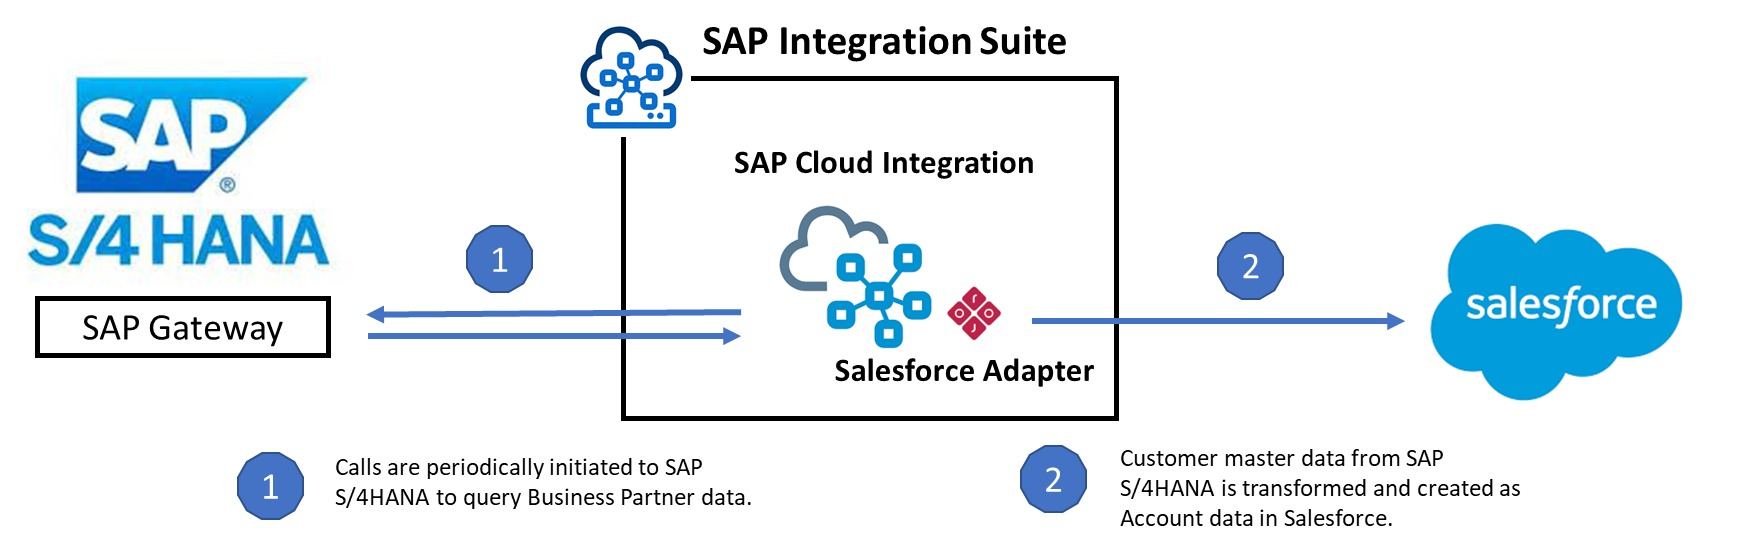
\includegraphics[width=0.8\textwidth]{Chapter4/Pictures/Arct_ov.jpg}}
    \caption{Overview of System Architecture}
    \label{fig:impl}
\end{figure}

\subsection{Prerequisites}

To successfully configure the integration content as described in this guide, it is imperative to ensure that you have the necessary access rights and authorizations for the systems involved. This configuration is pivotal for establishing a robust integration between SAP S/4HANA and Salesforce, leveraging BTP Middleware, specifically SAP Cloud Platform Integration (CPI). Below is a detailed breakdown of the access and authorization requirements for each system.

\subsubsection{Access Requirements}
\begin{itemize}
    \item \textbf{SAP S/4HANA Tenant Details:}
    \begin{itemize}
        \item You must have access to the SAP S/4HANA system, which serves as the core ERP platform for managing business processes.
        \item Ensure connectivity to the SAP S/4HANA tenant, as it will act as the source or target system for data exchange during the integration process.
    \end{itemize}

        \begin{figure}[H]
    \centering
    \fbox{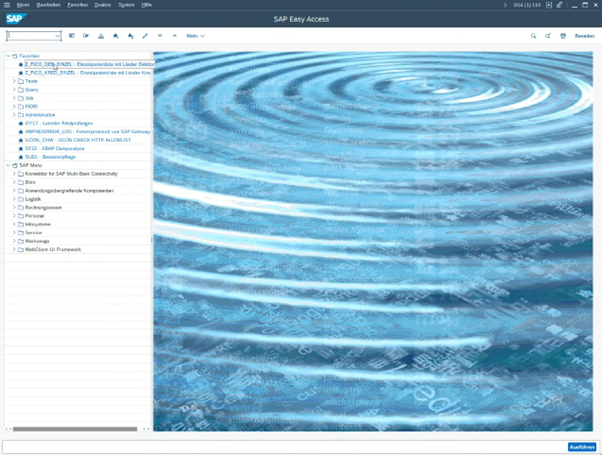
\includegraphics[width=0.8\textwidth]{Chapter4/Pictures/s4hana.png}}
    \caption{S4 Hana Home Page}
    
\end{figure}

    \item \textbf{SAP Cloud Platform Integration (CPI) Tenant Details:}
    \begin{itemize}
        \item Access to the SAP CPI tenant is required, as it functions as the middleware facilitating the integration between SAP S/4HANA and Salesforce.
        \item The CPI tenant will host the integration flows, mappings, and transformations necessary for seamless DS.
    \end{itemize}

\begin{figure}[H]
    \centering
    \fbox{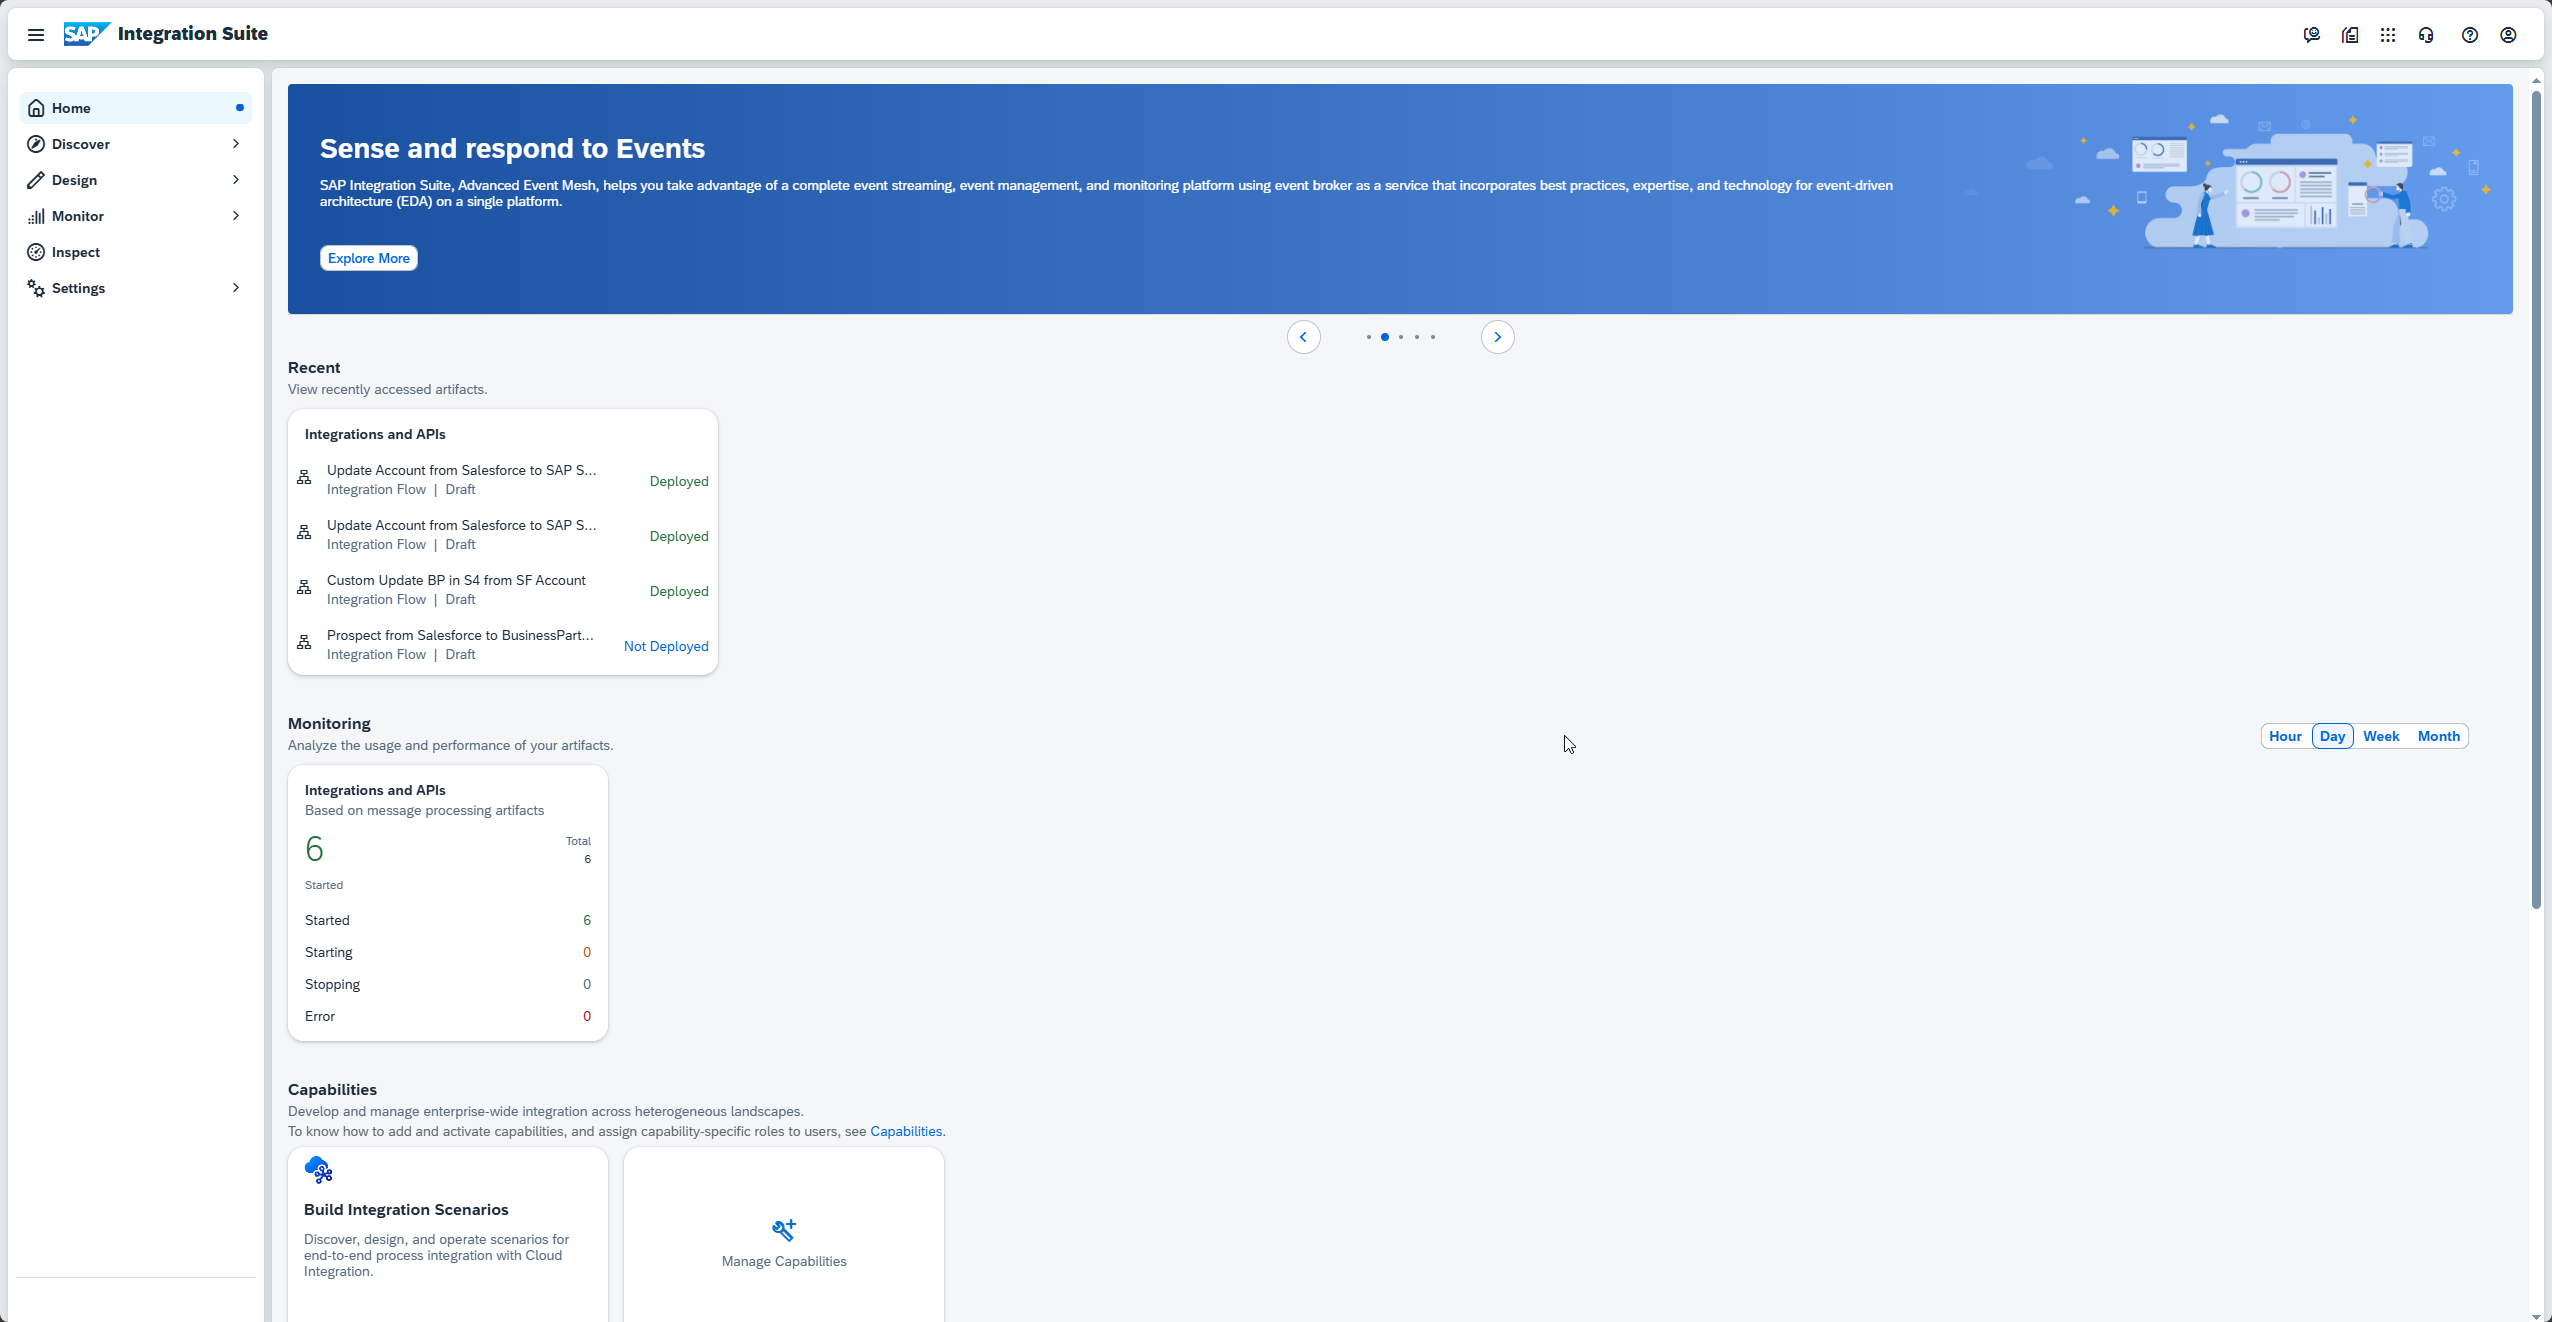
\includegraphics[width=0.8\textwidth]{Chapter4/Pictures/integrationsuite.png}}
    \caption{Integration Suite Home Page}
    
\end{figure}
    

    \item \textbf{Salesforce Tenant Details:}
    \begin{itemize}
        \item Access to the Salesforce tenant is essential, as it serves as the CRM platform where customer, product, and sales-related data will be synchronized.
        \item Ensure connectivity to the Salesforce environment to enable bidirectional data exchange with SAP S/4HANA.
    \end{itemize}
\end{itemize}


\begin{figure}[H]
    \centering
    \fbox{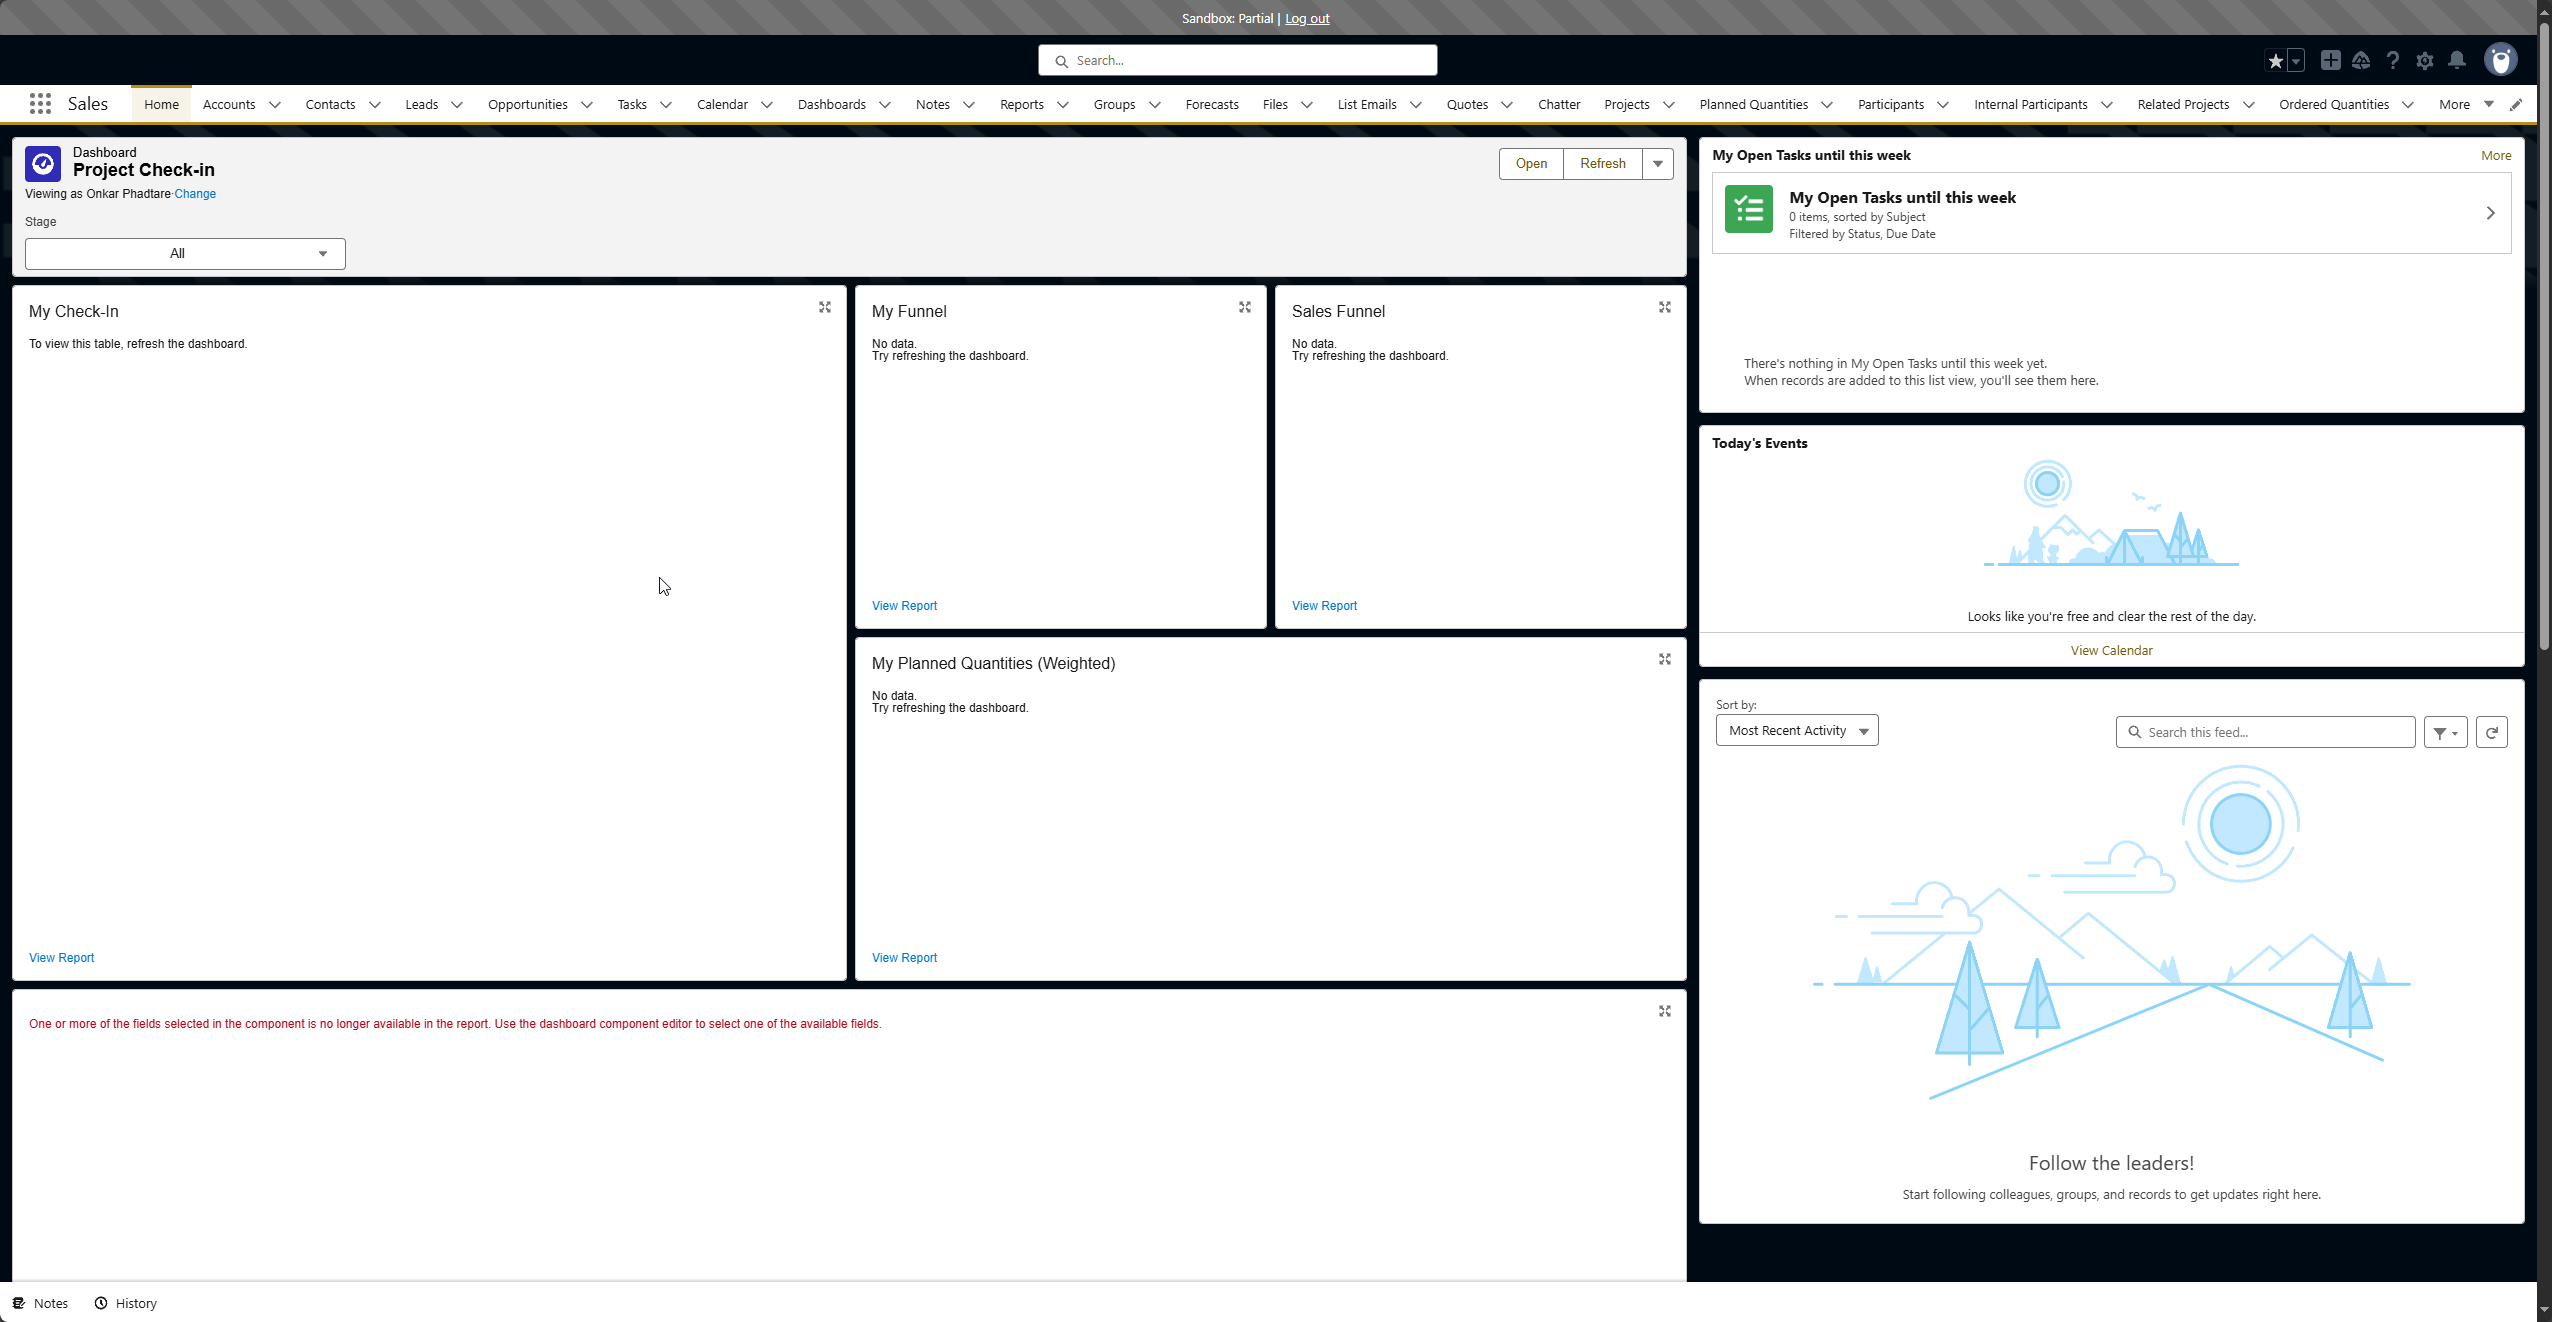
\includegraphics[width=0.8\textwidth]{Chapter4/Pictures/salesforce.png}}
    \caption{Salesforece Home Page}
    
\end{figure}

\subsubsection{Authorization Requirements}
\begin{itemize}
    \item \textbf{SAP S/4HANA Tenant Details:}
    \begin{itemize}
        \item \textbf{Access to SAP Gateway:} You must have permissions to access the SAP Gateway, which enables the exposure of OData services required for data extraction and integration.
        \item \textbf{User Creation and Role Assignment:} You need the ability to create users and assign appropriate roles within the SAP S/4HANA system to ensure secure and authorized access to data.
        \item \textbf{Access to Master Data (Product Master):} Permissions to access and manage Product Master data are necessary, as this data will be synchronized with Salesforce.
        \item \textbf{Access to Sales Master Data:} You must have access to Sales Master Data, which includes customer and pricing information, to facilitate accurate data exchange.
        \item \textbf{Access to Sales Order Data:} Permissions to access Sales Order data are required, as this information may need to be shared or updated between SAP S/4HANA and Salesforce.
    \end{itemize}

    

    \item \textbf{SAP Cloud Platform Integration (CPI) Tenant Details:}
    \begin{itemize}
        \item \textbf{Authorization Group (\texttt{AuthGroup.IntegrationDeveloper}):} You must be assigned the \texttt{AuthGroup.IntegrationDeveloper} role within SAP CPI to design, configure, and deploy integration flows. This role grants the necessary permissions to create and manage integration artifacts, such as mappings, transformations, and adapters.
    \end{itemize}

    \begin{figure}[H]
    \centering
    \fbox{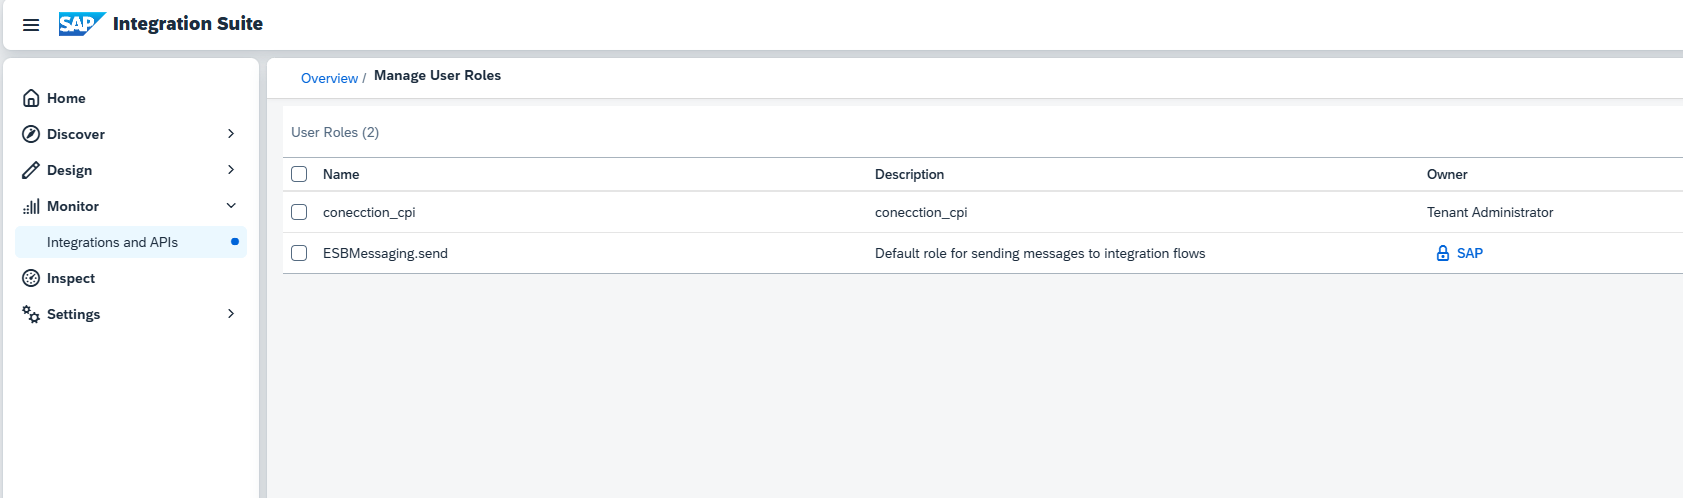
\includegraphics[width=0.8\textwidth]{Chapter4/Pictures/integrationrole.png}}
    \caption{SAP Cloud Platform Integration (CPI) Tenant Details:}
    
    \end{figure}

    \item \textbf{Salesforce Tenant:}
    \begin{itemize}
        \item \textbf{Appropriate Permissions for Configuration:} You must have sufficient permissions within the Salesforce tenant to configure and manage the integration. This includes the ability to create and modify Custom Fields for specific Salesforce objects (e.g., Account, Contact, Opportunity) that will be involved in the integration.
        \item \textbf{Access to Salesforce APIs:} Ensure that you have access to Salesforce APIs, as they will be used to send and retrieve data between Salesforce and SAP CPI.
        \item \textbf{Permission to Manage Integration User:} You may need to create or configure an integration user in Salesforce with the necessary permissions to allow data exchange with SAP CPI.
    \end{itemize}
\end{itemize}


The successful configuration and operation of the integration between SAP S/4HANA and Salesforce via SAP BTP Middleware (CPI) depend on fulfilling the access and authorization requirements outlined above. These prerequisites ensure that the integration flows can be designed, deployed, and executed seamlessly, enabling efficient DS and process automation across the two platforms. Proper configuration of both systems, along with the necessary permissions, is critical to achieving a robust and reliable integration solution.

\subsection{Adapter Installation }
The configuration of the Salesforce Adapter within the SAP Cloud Platform Integration (CPI) is a critical step in enabling seamless and secure data exchange between Salesforce and SAP S/4HANA. SAP CPI serves as an intermediary platform that facilitates the integration of business-critical data across these systems. To ensure secure and efficient communication, Salesforce employs an OAuth-based authentication mechanism, which provides a robust framework for secure API access. The configuration process involves two primary components: the installation of the Salesforce Adapter and the establishment of authentication mechanisms. Below is a detailed elaboration of these steps.

\begin{enumerate}
    \item \textbf{Installing the Salesforce Adapter} \\
    The Salesforce Adapter is a specialized integration component that enables connectivity between SAP CPI and Salesforce. Its installation is a prerequisite for creating integration flows that leverage Salesforce APIs. The installation process involves the following steps:
    \begin{itemize}
        \item Download the Salesforce Adapter package in .zip format from the appropriate source.
        \item Log into the SAP CPI Integration Suite and navigate to the \textit{Design} section, followed by \textit{Integration Suite}.
        \item Select the \textit{Edit} option and choose \textit{Add Integration Adapter} to initiate the installation process.
        \item Upload the downloaded Salesforce Adapter package in .zip format.
        \item Confirm the installation by clicking \textit{OK}.
        \item Navigate to \textit{Integration Monitor} and select \textit{Manage Integration Content} to verify the adapter's availability.
        \item Deploy the adapter to activate it for use in integration flows.
    \end{itemize}
    Upon successful deployment, the Salesforce Adapter becomes operational and can be utilized to design and execute integration flows between SAP CPI and Salesforce.

    \item \textbf{Establishing Authentication with Salesforce} \\
    To ensure the secure transfer of data, authentication credentials must be configured within SAP CPI. This involves setting up two distinct authentication mechanisms: Salesforce User Authentication and OAuth Authentication for the Salesforce Connected App. The steps for each are outlined below:
    \begin{itemize}
        \item \textbf{Salesforce User Authentication}:
        \begin{itemize}
            \item Navigate to the \textit{Security} section in SAP CPI and select \textit{Create Credentials}.
            \item Enter the following details:
            \begin{itemize}
                \item \textit{Username}: The email address associated with the Salesforce account.
                \item \textit{Password}: The password for the Salesforce account.
            \end{itemize}
            \item Click \textit{Deploy} to finalize the configuration.
        \end{itemize}
        \item \textbf{OAuth Authentication for Salesforce Connected App}:
        \begin{itemize}
            \item In Salesforce, create a \textit{Connected App} to generate OAuth credentials, including the \textit{Consumer Key}, \textit{Consumer Secret}, and \textit{Security Token}. The security token is typically sent to the registered email address.
            \item Copy the generated OAuth credentials from the Connected App.
            \item Return to SAP CPI and navigate to the \textit{Security} section, then select \textit{Create Credentials}.
            \item Configure the OAuth Client Credentials using the copied values from the Connected App.
            \item Deploy the credentials to establish a secure connection between SAP CPI and Salesforce.
        \end{itemize}
    \end{itemize}
    Once these authentication mechanisms are configured, SAP CPI can securely authenticate API requests to Salesforce, ensuring the protected exchange of business-critical data.
\end{enumerate}

In summary, the configuration of the Salesforce Adapter in SAP CPI involves a systematic approach to installing the adapter and establishing secure authentication mechanisms. This process ensures that the integration between Salesforce and SAP S/4HANA is both efficient and secure, enabling organizations to leverage their data effectively while maintaining compliance with security standards.


\section{Configuration}

Before the integration content package can be configured and deployed, it is essential to ensure that the respective systems SAP S/4HANA, Salesforce, and SAP Cloud Platform Integration (CPI) are properly configured and prepared. This preparatory phase involves establishing the necessary technical and operational prerequisites to facilitate seamless data exchange and process automation between the systems. The configuration process requires meticulous attention to system settings, access permissions, and connectivity parameters to ensure compatibility and functionality. Detailed steps for achieving this configuration are outlined in the subsequent sections of this guide. These steps provide a structured approach to preparing the systems, enabling the successful deployment and execution of the integration content package.

\subsection{Configuration in SAP S/4HANA }

This section outlines the essential configurations that must be executed within the SAP S/4HANA system as a prerequisite to initiating the implementation of Salesforce-related configurations or the setup of integration content in SAP Cloud Platform Integration (CPI). These mandatory configurations are critical to ensuring that the SAP S/4HANA system is fully prepared to support seamless data exchange and process integration with Salesforce and SAP CPI. The steps detailed in the subsequent sub-sections provide a systematic and comprehensive guide to completing these configurations, thereby establishing a robust foundation for the integration process. Adherence to these steps is imperative to achieve compatibility, functionality, and operational efficiency across the integrated systems.

\subsubsection{Create Technical Communication User }

A Technical Communication User is a prerequisite for enabling the invocation of OData services in SAP S/4HANA from SAP Cloud Platform Integration (CPI). This user serves as a dedicated entity for facilitating inbound communication and processing messages within the SAP S/4HANA system. The creation of such a user is a critical step in establishing secure and authorized communication between SAP S/4HANA and external systems, such as SAP CPI, during the integration process. Below is a detailed procedural guide for creating a communication user in SAP S/4HANA.

\paragraph{Procedure}
\begin{enumerate}
    \item \textbf{Access the Transaction Code:}
    \begin{itemize}
        \item Launch the SAP GUI and enter the transaction code \texttt{SU01} to access the User Maintenance interface.
    \end{itemize}

    \item \textbf{User Maintenance Initial Screen:}
    \begin{itemize}
        \item On the initial screen, input the desired \texttt{<User ID>} in the designated field. This ID will uniquely identify the technical communication user.
    \end{itemize}

    \item \textbf{Initiate User Creation:}
    \begin{itemize}
        \item Select the "Create" option to proceed with the creation of a new user.
    \end{itemize}

    \item \textbf{Maintain User Details:}
    \begin{itemize}
        \item Navigate to the "Maintain User" screen and populate the required fields with the following values:
        \begin{itemize}
            \item \textbf{Last Name:} Provide a descriptive name for the user.
            \item \textbf{Logon Data Tab:}
            \begin{itemize}
                \item Set the \textbf{User Type} to "Communication Data" to designate the user as a technical communication user.
                \item Assign a secure \texttt{<password>} to ensure authentication.
            \end{itemize}
        \end{itemize}
        \item \textbf{Note:} It is imperative to assign the user appropriate authorizations to enable the execution of OData API calls. These authorizations are essential for the user to interact with OData services effectively.
    \end{itemize}

    \item \textbf{Save the Configuration:}
    \begin{itemize}
        \item Once all fields have been populated, click the "Save" button to finalize the creation of the technical communication user.
    \end{itemize}
\end{enumerate}

The creation of a technical communication user is a foundational step in the integration process, as it ensures secure and authorized access to SAP S/4HANA's OData services. This user acts as a bridge between SAP S/4HANA and SAP CPI, enabling the seamless exchange of data and the execution of integration workflows. Proper configuration and authorization of this user are critical to maintaining system security, operational efficiency, and compliance with integration requirements.

    \begin{figure}[H]
    \centering
    \fbox{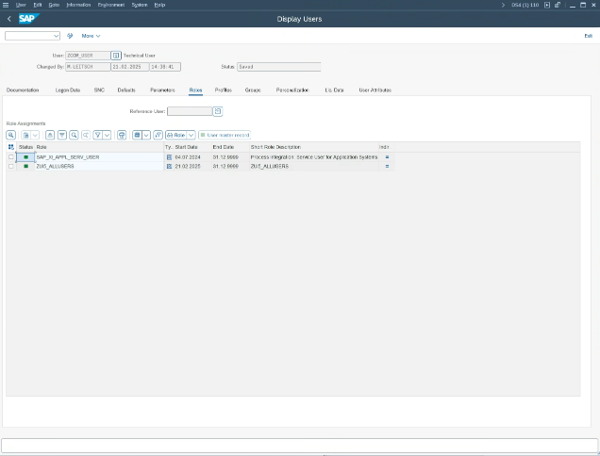
\includegraphics[width=0.8\textwidth]{Chapter4/Pictures/s4hana_role.png}}
    \caption{S4 HANA Communication user}
    
\end{figure}


\subsubsection{Activating SAP Gateway }

Before utilizing the SAP Gateway functionality, it is essential to ensure that it is globally activated within the SAP S/4HANA system. SAP Gateway serves as a critical component for enabling OData services, which facilitate communication between SAP S/4HANA and external systems, such as SAP Cloud Platform Integration (CPI). If SAP Gateway is not activated, OData services will not function, resulting in communication failures between consumer servers and the SAP system. In such cases, any system attempting to call these services will receive an error message. 

The activation process involves configuration activities that can be performed via the SAP Reference IMG (transaction code: \texttt{SPRO}). Specifically, the configuration settings are located under the path: \texttt{SAP NetWeaver > SAP Gateway > OData Channel > Configuration > User Settings and Connection Settings}. Once these configurations are completed, SAP Gateway must be activated using the steps outlined below.

\paragraph{Procedure}
\begin{enumerate}
    \item \textbf{Access the SAP Reference IMG:}
    \begin{itemize}
        \item Launch the SAP GUI and enter the transaction code \texttt{SPRO} to access the SAP Reference IMG.
    \end{itemize}

    \item \textbf{Navigate to SAP Gateway Configuration:}
    \begin{itemize}
        \item Within the SAP Reference IMG, navigate to the following path: \\
        \texttt{SAP NetWeaver > SAP Gateway > OData Channel > Configuration > Activate or Deactivate SAP Gateway}.
        \item Click on the "Activity" icon to proceed. A confirmation message will be displayed.
    \end{itemize}

    \item \textbf{Activate SAP Gateway:}
    \begin{itemize}
        \item Select the "Activate" option to enable SAP Gateway. Upon activation, a message will be displayed to confirm the current status of SAP Gateway.
    \end{itemize}
\end{enumerate}

The activation of SAP Gateway is a fundamental step in enabling OData services, which are essential for seamless communication between SAP S/4HANA and external systems. Without activation, OData services remain non-functional, leading to communication failures and disruptions in integration workflows. Proper activation ensures that consumer servers can interact with SAP S/4HANA effectively, facilitating data exchange and process automation. This step is critical for maintaining system functionality, operational efficiency, and compliance with integration requirements.


\subsubsection{Activate OData API in Gateway}
The integration between Salesforce and SAP S/4HANA relies on the OData APIs provided by SAP S/4HANA. These APIs serve as the foundation for enabling seamless data exchange and process automation between the two systems. To facilitate this integration, the relevant OData APIs must be activated in SAP Gateway. This section provides a detailed procedural guide for activating the OData APIs required by the integration content.

\paragraph{Procedure}
\begin{enumerate}
    \item \textbf{Access the Transaction Code:}
    \begin{itemize}
        \item Launch the SAP GUI and enter the transaction code \texttt{/IWFND/MAINT\_SERVICE}. This transaction displays the Service Catalog, which lists all activated Gateway services in the target system and allows for the addition of new services.
    \end{itemize}

    \item \textbf{Add a New Service:}
    \begin{itemize}
        \item Click the "Add Service" button located in the toolbar to initiate the process of adding a new service.
    \end{itemize}

    \item \textbf{Enter System Alias:}
    \begin{itemize}
        \item Input the System Alias of your front-end server in the designated field.
    \end{itemize}

    \item \textbf{Enter External Service Name:}
    \begin{itemize}
        \item Specify the External Service Name as \texttt{API\_BUSINESS\_PARTNER}.
    \end{itemize}

    \item \textbf{Retrieve Available Services:}
    \begin{itemize}
        \item Click the "Get Services" button in the toolbar to retrieve the list of available services. The requested service will be displayed for selection.
    \end{itemize}

    \item \textbf{Select and Add the Service:}
    \begin{itemize}
        \item Select the service generated from the previous step and click "Add Selected Services" or use the object link for further selection.
    \end{itemize}

    \item \textbf{Configure Technical Service Details:}
    \begin{itemize}
        \item In the "Add Service" dialog, the system will suggest the Technical Service name as \texttt{ZAPI\_BUSINESS\_PARTNER} and the Technical Model. The dialog will also indicate that the model metadata for the Gateway service is being created.
    \end{itemize}

    \item \textbf{Specify the Package:}
    \begin{itemize}
        \item Assign a package for the service activation process.
    \end{itemize}

    \item \textbf{Complete the Configuration:}
    \begin{itemize}
        \item Leave the remaining fields in the dialog unchanged and click "Continue." A confirmation dialog will appear, indicating that the model metadata for the Gateway service has been successfully created.
    \end{itemize}

    \item \textbf{Repeat for Additional APIs:}
    \begin{itemize}
        \item Repeat the above steps to activate the following additional APIs:
        \begin{itemize}
            \item \texttt{API\_SALES\_CONTRACT\_SRV}
            \item \texttt{API\_SALES\_ORDER\_SRV}
        \end{itemize}
    \end{itemize}
\end{enumerate}


The activation of OData APIs in SAP Gateway is a critical step in enabling the integration between Salesforce and SAP S/4HANA. These APIs provide the necessary interfaces for data exchange and process synchronization, ensuring seamless communication between the two systems. Proper activation and configuration of the APIs are essential for maintaining system functionality, operational efficiency, and compliance with integration requirements. This process lays the foundation for robust and reliable integration workflows, facilitating automation and data consistency across platforms.


\subsection{Configuration in Salesforce.com  }

This section delineates the mandatory configurations required within Salesforce to establish a robust integration framework with SAP S/4HANA. These configurations encompass the setup of Security Tokens and OAuth Credentials, which are essential for ensuring secure and authenticated communication between Salesforce and external systems such as SAP Cloud Platform Integration (CPI). Additionally, the creation of Custom Fields, designated as External IDs, is necessary to store unique identifiers from SAP S/4HANA, enabling accurate data mapping and synchronization. These preparatory tasks are critical prerequisites that must be completed before proceeding with the implementation and configuration of the integration content in SAP CPI. Proper execution of these configurations ensures the integrity, security, and efficiency of the integration process, facilitating seamless data exchange and process automation between Salesforce and SAP S/4HANA.

Security Tokens and OAuth Credentials are essential components for establishing a secure connection to Salesforce, enabling authenticated and authorized access to its data and services. To retrieve these credentials, an application must first be created within the Salesforce tenant. This application serves as the intermediary entity that facilitates secure communication between Salesforce and external systems, such as SAP Cloud Platform Integration (CPI). The process of obtaining the Security Token and OAuth Credentials involves configuring the application within Salesforce, generating the necessary tokens, and ensuring that the credentials are securely stored and managed. These steps are critical for maintaining the integrity and security of the integration, as they provide the foundation for secure data exchange and process automation between Salesforce and external platforms.

\subsubsection{Deploying OAuth}

The process of deploying OAuth within the SAP Cloud Platform Integration (CPI) tenant involves a series of structured steps to ensure proper configuration and security. Below is a detailed explanation of the procedure:

\begin{enumerate}
    \item \textbf{Access the Monitoring Section}: Begin by navigating to the "Monitor" section within your SAP CPI tenant. This section provides an overview of the integration flows and allows you to manage various operational aspects of the platform.

    \item \textbf{Navigate to Security Management}: Within the "Monitor" interface, locate and select the "Manage Security" option. This section is dedicated to configuring and maintaining security-related settings, ensuring that your integration flows are protected against unauthorized access.

    \item \textbf{Access Security Material}: Under the "Manage Security" menu, click on "Security Material." This subsection is where you can manage and store security artifacts, such as certificates, keys, and credentials, which are essential for secure communication and authentication.

    \item \textbf{Create User Credentials}: In the "Security Material" section, click on the "Add" dropdown menu and select "User Credentials." This action initiates the creation of a new set of credentials that will be used for authentication purposes.

    \item \textbf{Configure User Credentials}:
    \begin{itemize}
        \item \textbf{Name}: Assign a unique and identifiable name to the credentials for future reference. This name will help you easily locate and manage the credentials within the system.
        \item \textbf{User}: Input the OAuth token in the "User" field. This token serves as the authentication key, enabling secure access to the designated resources or services.
    \end{itemize}

    \item \textbf{Deploy the Configuration}: Once the credentials are properly configured, click on the "Deploy" button. This action finalizes the setup and activates the OAuth configuration, making it available for use in your integration flows.
\end{enumerate}

By following these steps, you ensure that the OAuth deployment is correctly implemented within your SAP CPI tenant, thereby enhancing the security and reliability of your integration processes.


\paragraph{Procedure}
To establish a secure connection to Salesforce, a Connected App must be created within the Salesforce tenant. This app facilitates the retrieval of Security Tokens and OAuth Credentials, which are essential for authenticated and authorized access to Salesforce data. The procedure is as follows:

\begin{enumerate}
    \item \textbf{Log in to Salesforce Console:}
    \begin{itemize}
        \item Access the Salesforce console and navigate to the \textbf{Setup} menu.
    \end{itemize}

    \item \textbf{Create a New Connected App:}
    \begin{itemize}
        \item From the left panel, under the \textbf{Build overview}, select \textbf{Create - Apps}, and then click \textbf{New} in the \textbf{Connected Apps} section (see Figure 4.1).
        \begin{figure}[h!]
            \centering
            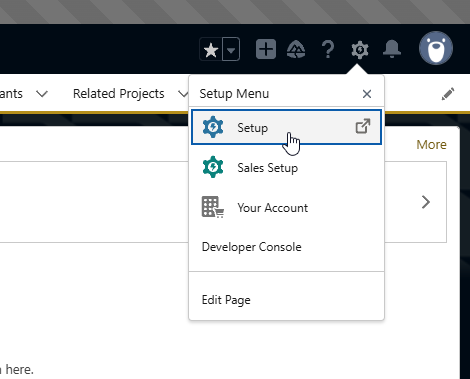
\includegraphics[width=0.8\textwidth]{Chapter4/Pictures/Setup.png} % Replace with actual figure file
            \caption{Salesforce Setup Menu}
            \label{fig:create_app1}
        \end{figure}

         \begin{figure}[h!]
            \centering
            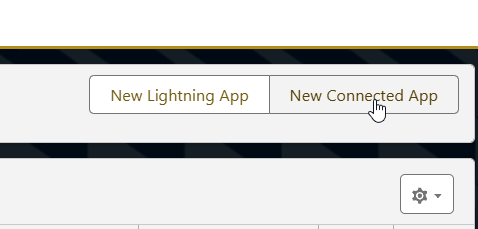
\includegraphics[width=0.8\textwidth]{Chapter4/Pictures/con_app.png} % Replace with actual figure file
            \caption{Creating a New Connected App in Salesforce}
            \label{fig:create_app2}
        \end{figure}
    \end{itemize}

    \item \textbf{Provide Basic Details:}
    \begin{itemize}
        \item On the next screen, fill in the required fields, including \textbf{App Name}, \textbf{API Name}, and \textbf{Contact Email}. Enable OAuth Settings by selecting the appropriate checkbox (see Figure 4.2).
        \begin{figure}[h!]
            \centering
            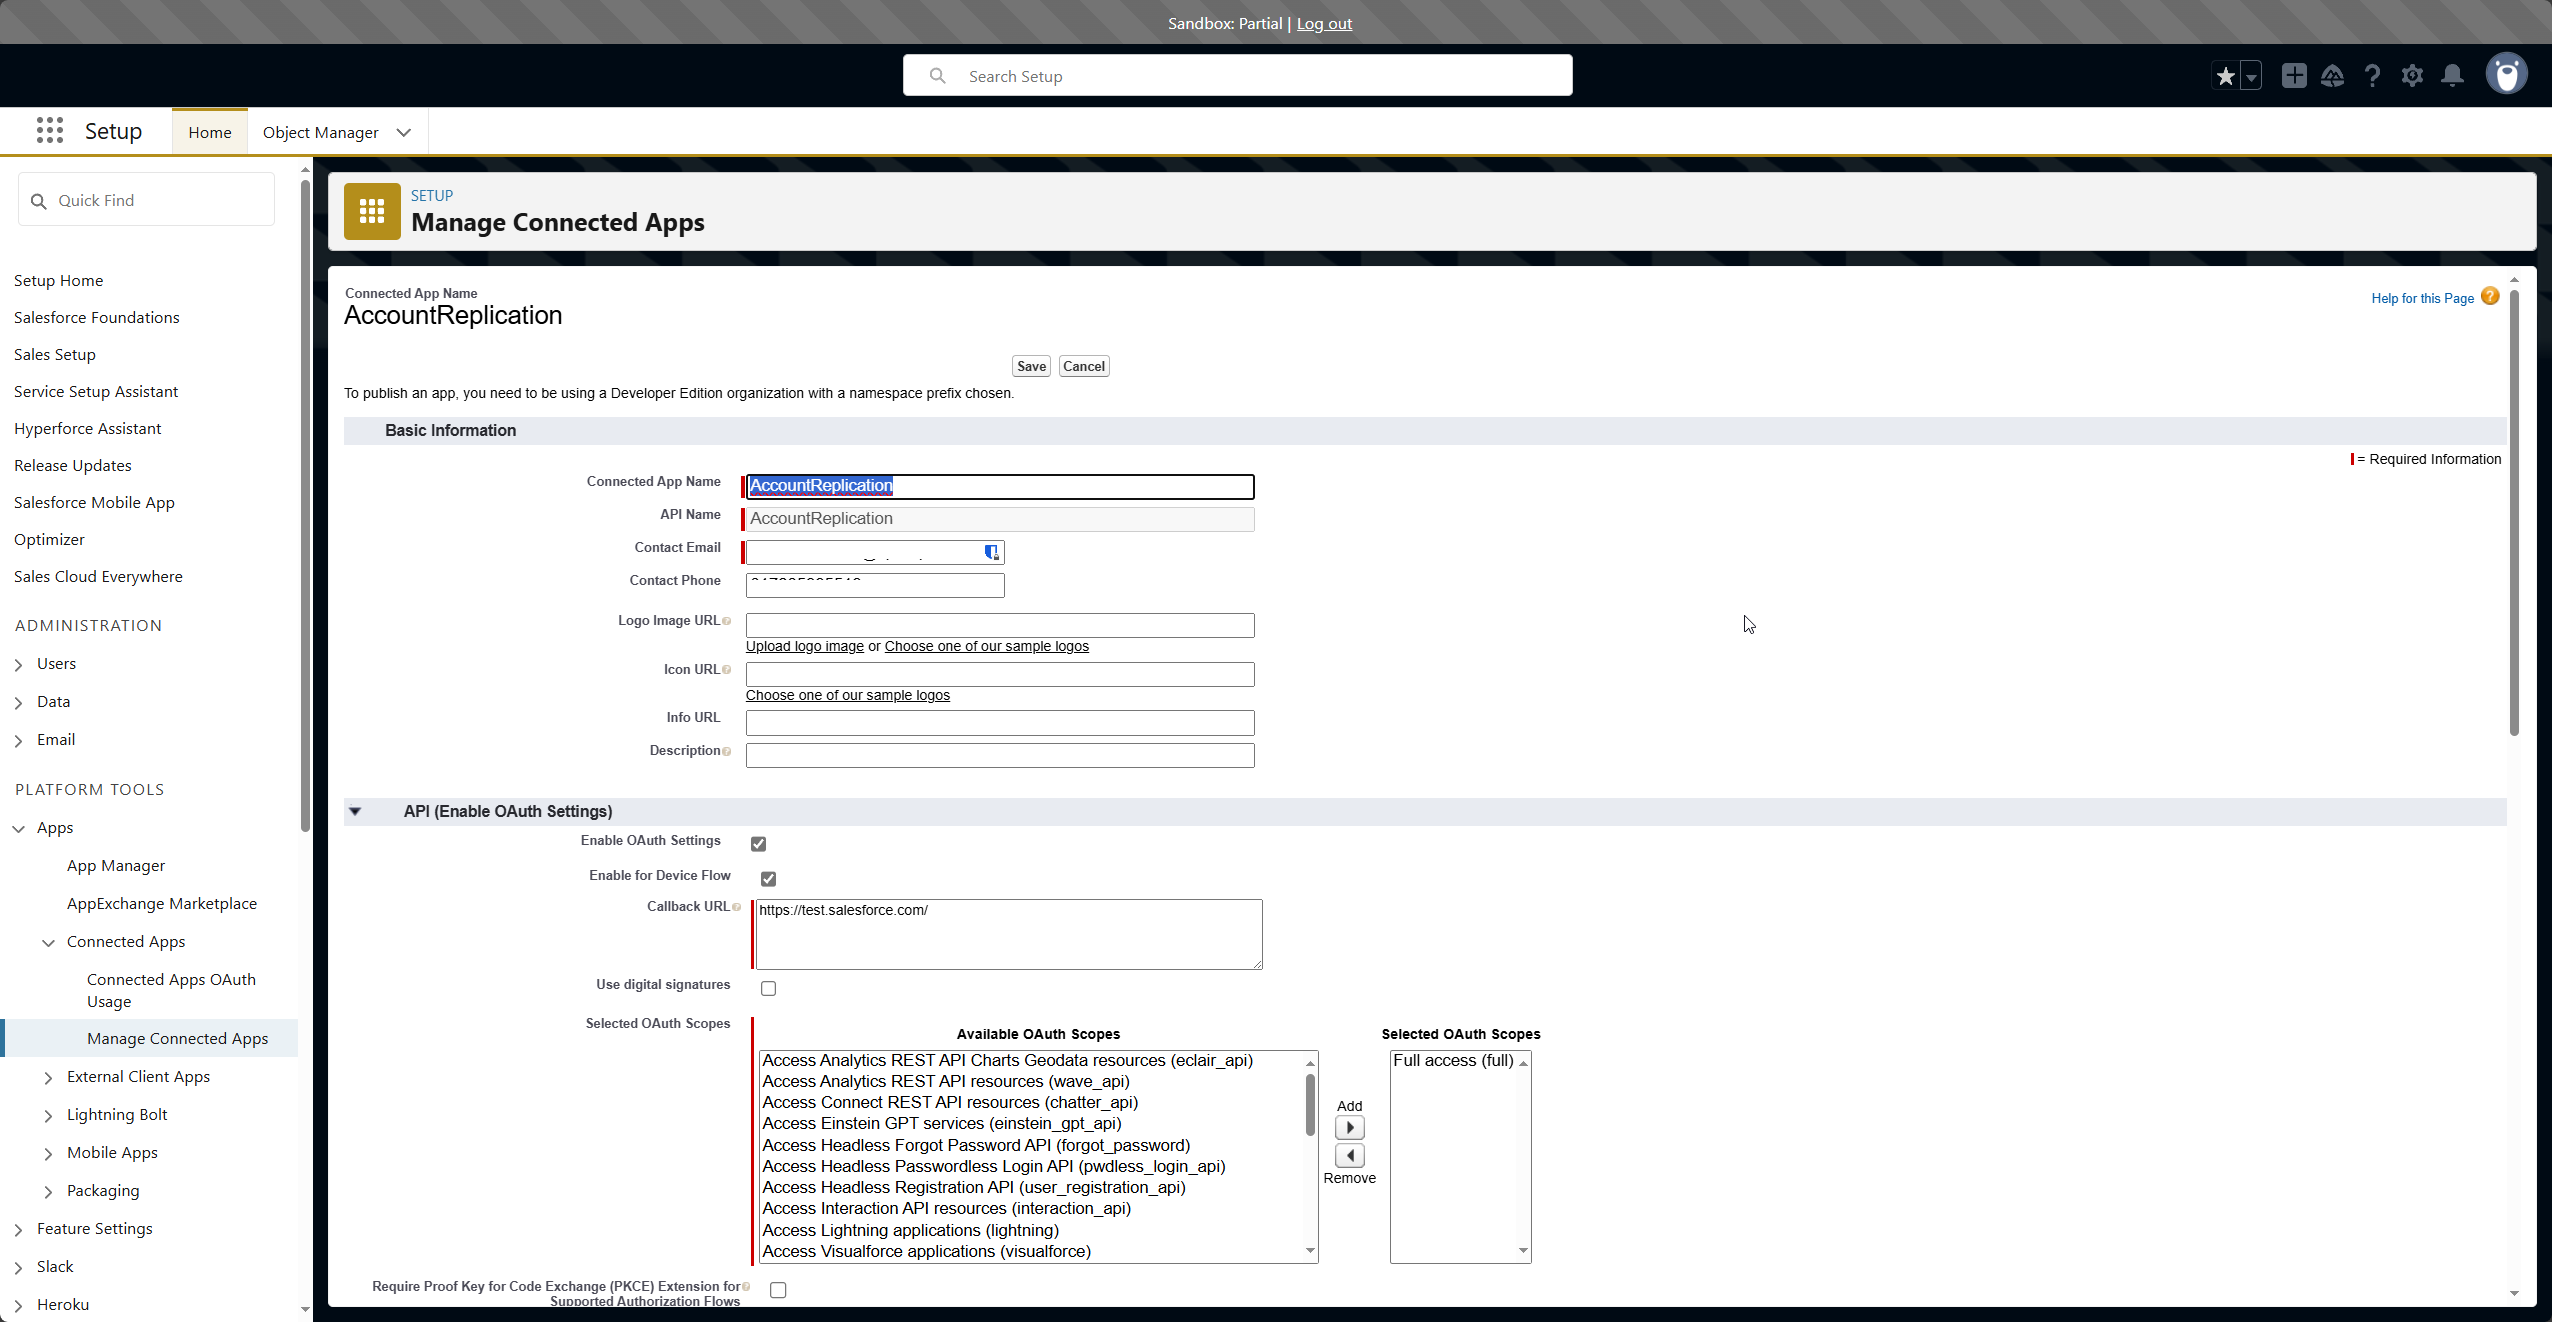
\includegraphics[width=0.8\textwidth]{Chapter4/Pictures/Connectedapp.png} % Replace with actual figure file
            \caption{Salesforce Connected App Configuration}
            \label{fig:new_app}
        \end{figure}
    \end{itemize}

    \item \textbf{Configure OAuth Settings:}
    \begin{itemize}
        \item In the API section (see Figure 4.3), perform the following actions:
        \begin{itemize}
            \item Disable \textbf{Enable for Device Flow}.
            \item Provide a \textbf{Callback URL}.
            \item Disable \textbf{Use digital signatures}.
            \item Set \textbf{Selected OAuth Scopes} to \textbf{Full access (full)}.
            \item Enable \textbf{Require Secret for Web Server Flow}.
            \item Disable \textbf{Include ID Token}.
            \item Disable \textbf{Enable Asset Tokens}.
        \end{itemize}
        \item Save the configuration to complete the creation of the Connected App.

    \end{itemize}

    \item \textbf{Retrieve Client ID and Client Secret:}
    \begin{itemize}
        \item Once the app is created, navigate to the app overview. The \textbf{Client ID} and \textbf{Client Secret} can be found in the \textbf{Consumer Key} and \textbf{Consumer Secret} fields, respectively (see Figure 4.4).

    \begin{figure}[H]
    \centering
    \fbox{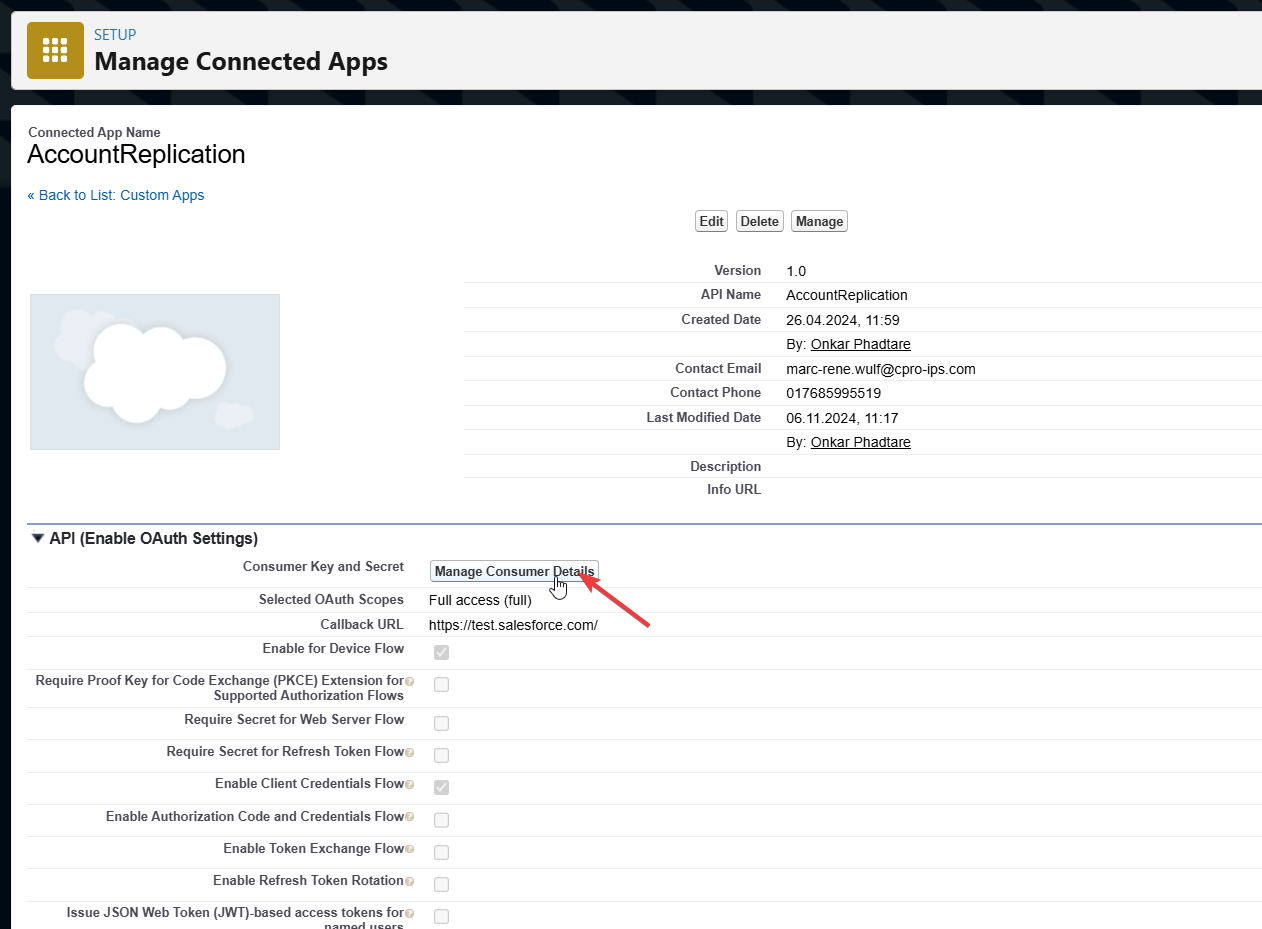
\includegraphics[width=0.8\textwidth]{Chapter4/Pictures/API.png}}
    \caption{OAuth Settings for Salesforce Connected App}
    
    \end{figure}

    \end{itemize}
\end{enumerate}


\subsubsection{Adding SAP S/4HANA References}
The integration content facilitates the synchronization of data between SAP S/4HANA Cloud and Salesforce. To achieve this, it is necessary to create unique identifiers in Salesforce that store key values from SAP S/4HANA Cloud. These identifiers, referred to as External IDs, enable accurate mapping and synchronization of records between the two systems. The following procedure outlines the steps required to add these references in Salesforce.

\paragraph{Procedure}
\begin{enumerate}
    \item \textbf{Access the Setup Screen:}
    \begin{itemize}
        \item Navigate to the Salesforce Setup menu to begin the configuration process.
    \end{itemize}

    \item \textbf{Locate the Object Fields:}
    \begin{itemize}
        \item In the Quick Find search box, type \texttt{Accounts*} and select \texttt{Fields} from the search results.
    \end{itemize}

    \begin{figure}[H]
    \centering
    \fbox{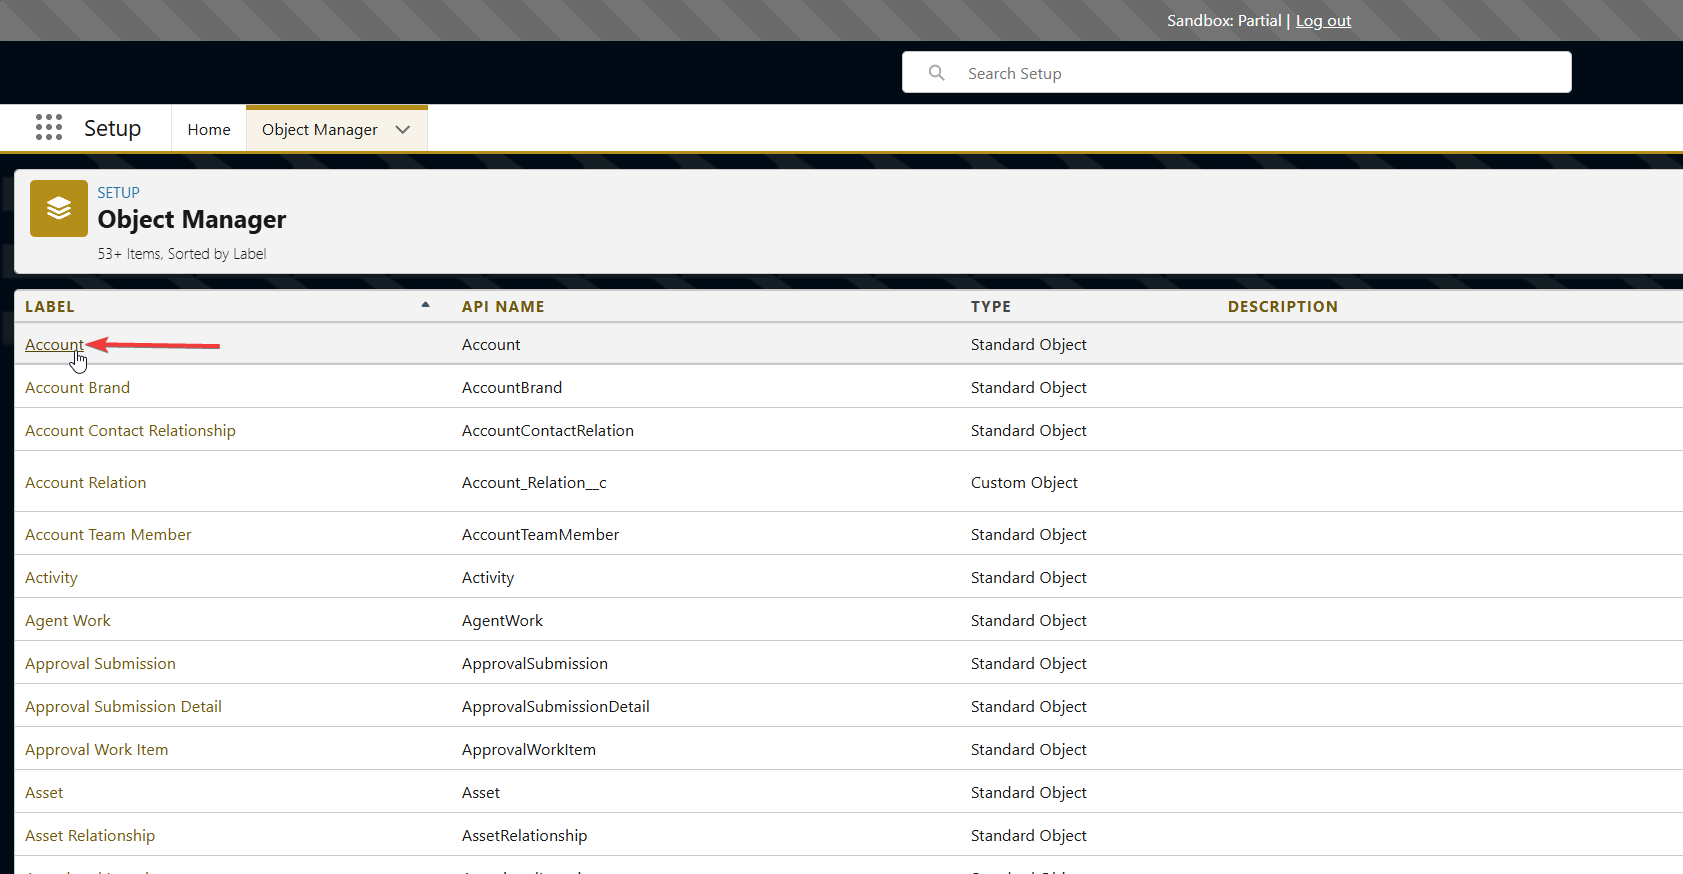
\includegraphics[width=0.8\textwidth]{Chapter4/Pictures/fieldsetup.png}}
    \caption{Salesforce Object Manager}
    
    \end{figure}

    \item \textbf{Create a New Field:}
    \begin{itemize}
        \item Scroll down and click the \texttt{New} button to initiate the creation of a new custom field.
    \end{itemize}

    \item \textbf{Select Field Type:}
    \begin{itemize}
        \item Choose \texttt{Text} as the field type and proceed by clicking \texttt{Next}.
    \end{itemize}

    \item \textbf{Define Field Properties:}
    \begin{itemize}
        \item Enter the field name as \texttt{SAP\_BusinessPartner\_Ref}, specify a length of \texttt{30 characters}, and enable the \texttt{External ID} checkbox. This ensures that the field can uniquely identify records from SAP S/4HANA Cloud.
    \end{itemize}
    
    \begin{figure}[H]
    \centering
    \fbox{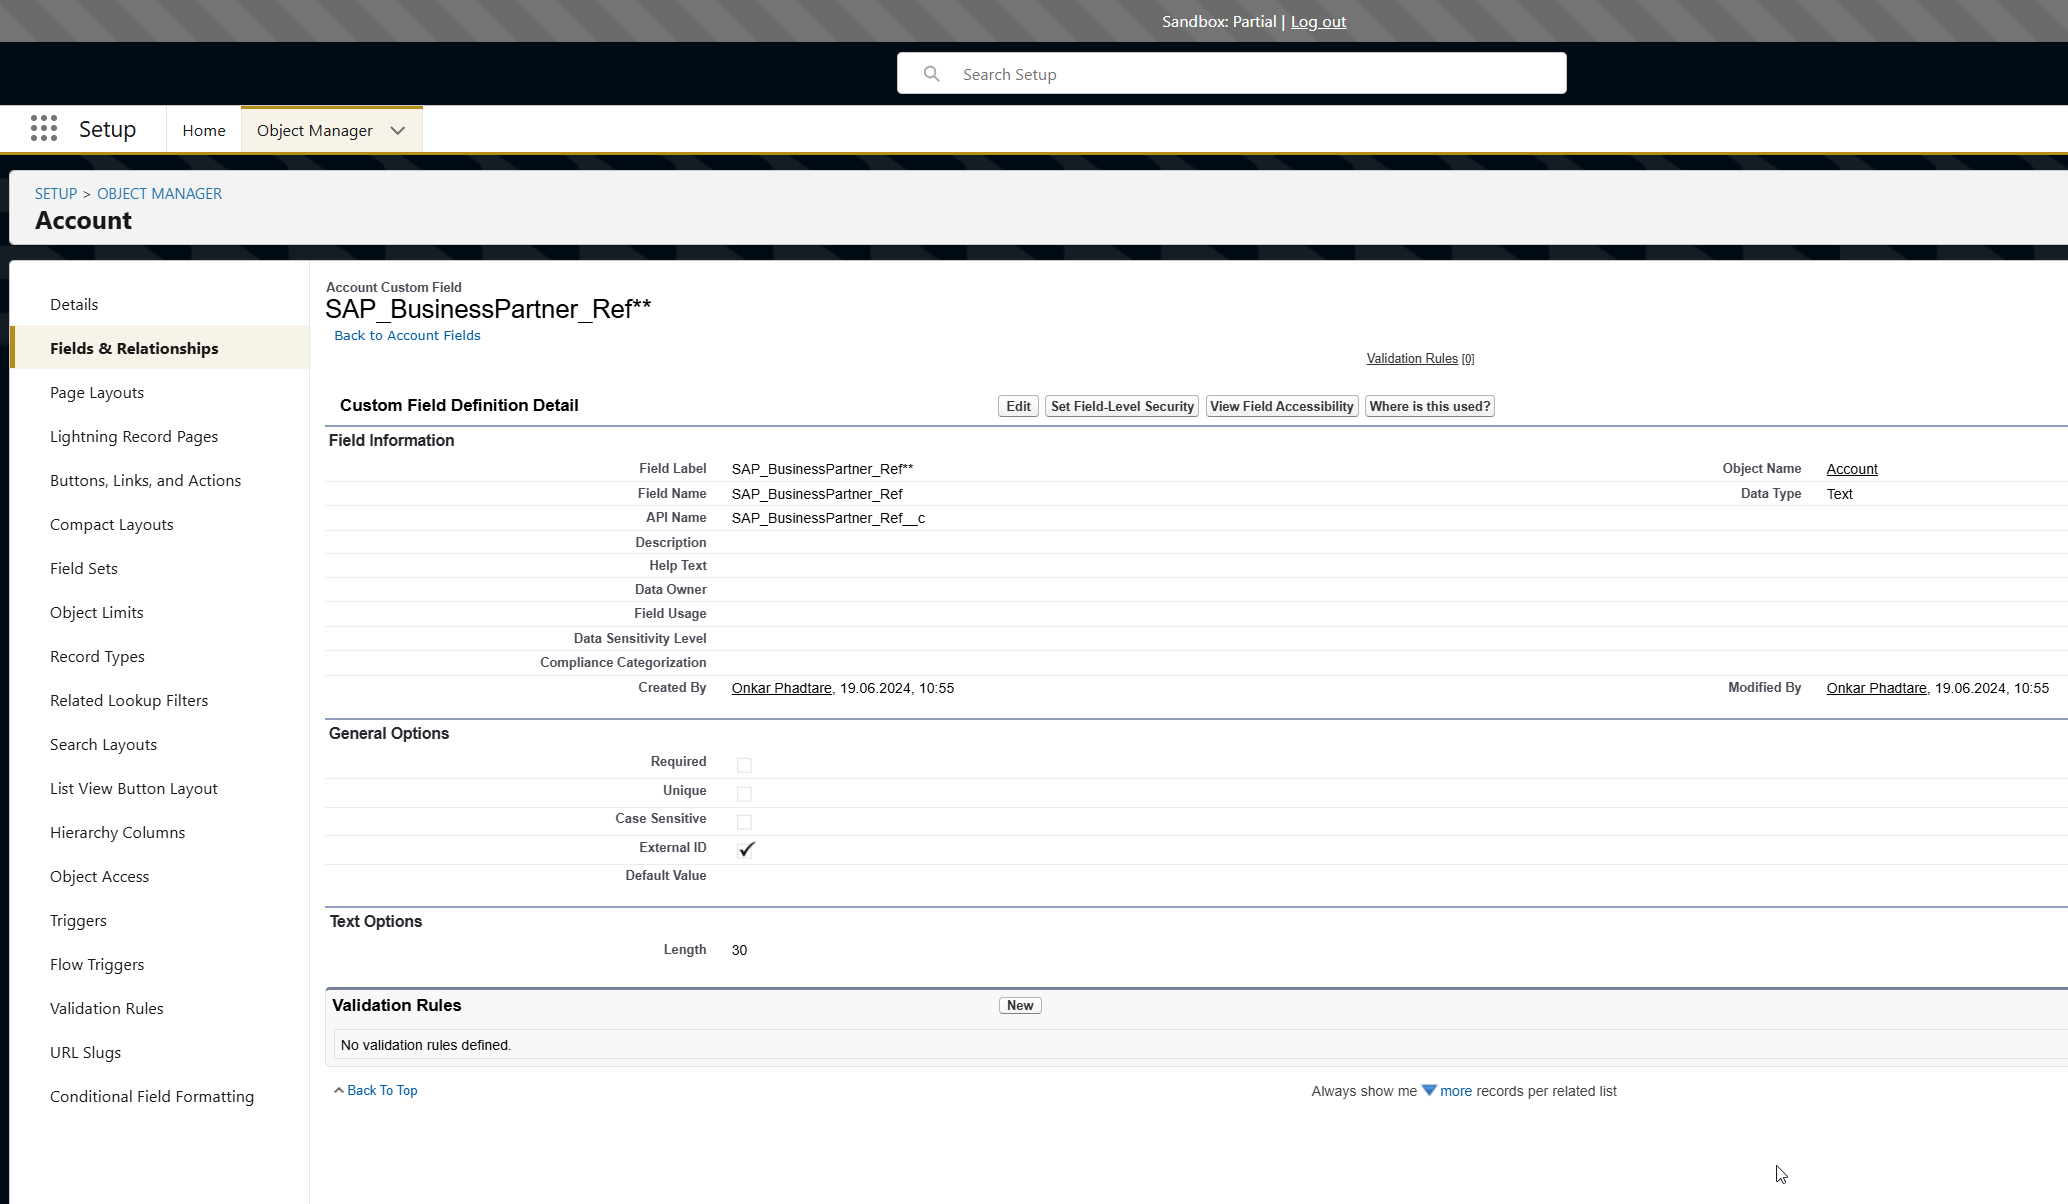
\includegraphics[width=0.8\textwidth]{Chapter4/Pictures/fieldlen.png}}
    \caption{Reference Field Details}
    
    \end{figure}
    

    \item \textbf{Complete Field Creation:}
    \begin{itemize}
        \item Click \texttt{Next} twice to proceed through the configuration screens, and then save the field.
    \end{itemize}

    \begin{figure}[H]
    \centering
    \fbox{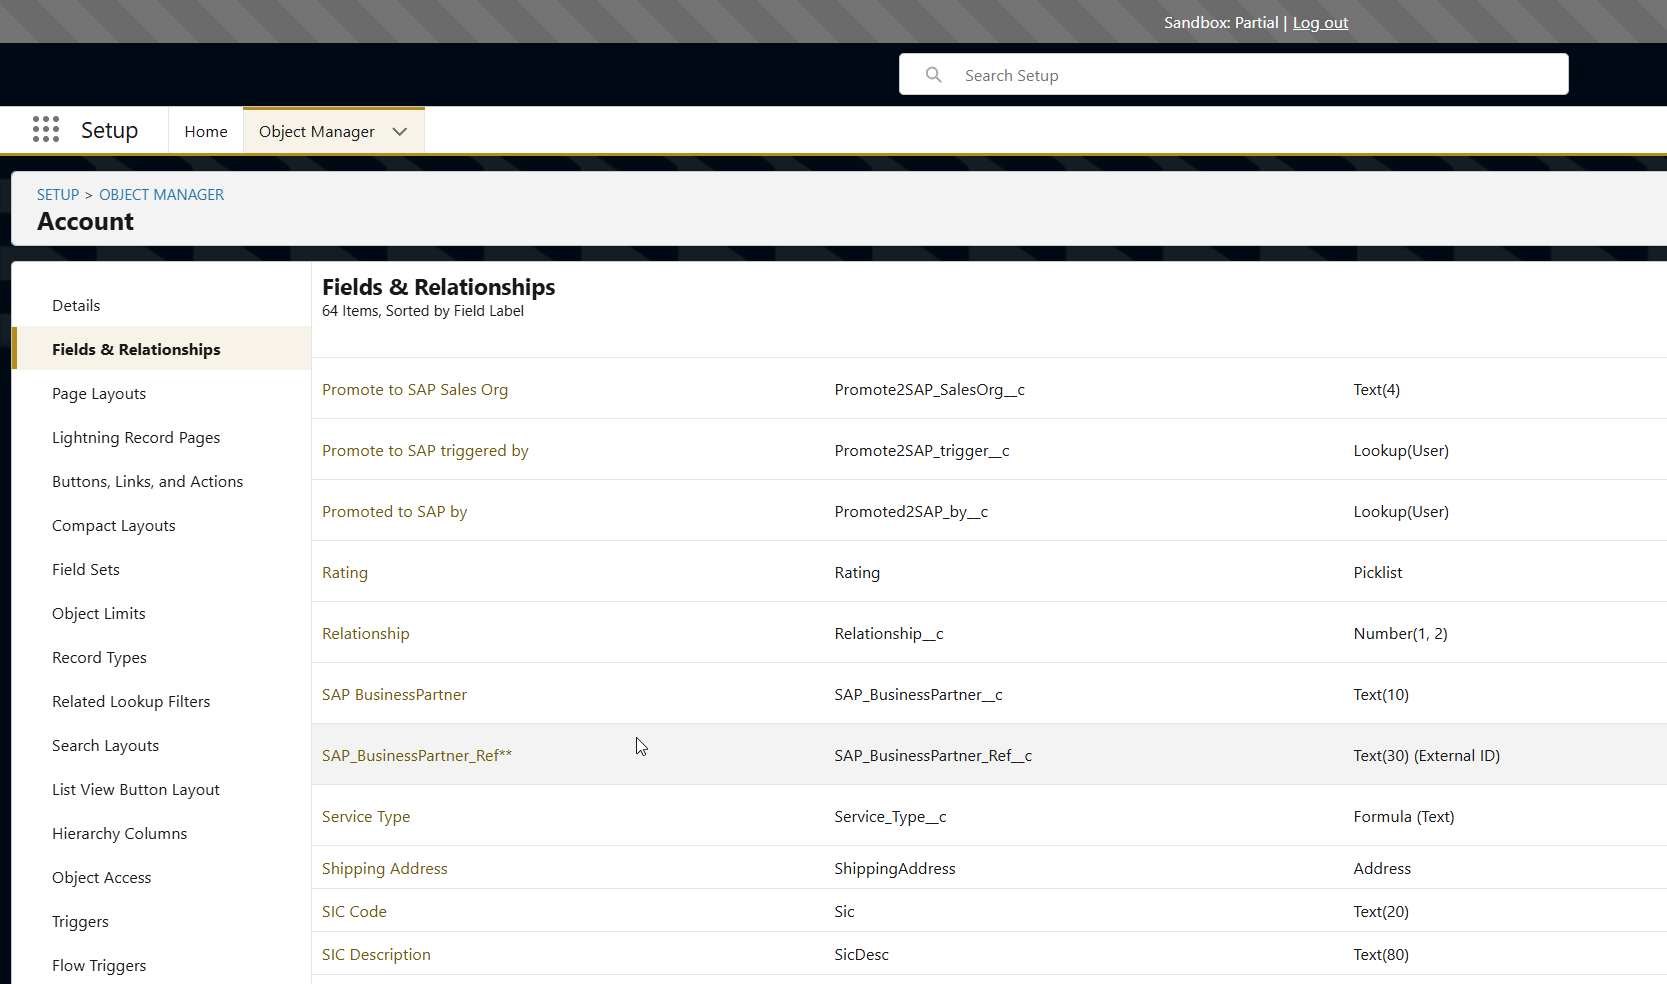
\includegraphics[width=0.8\textwidth]{Chapter4/Pictures/ref.png}}
    \caption{SAP BTP Integration Flow for Account Replication}
    
    \end{figure}

    \item \textbf{Repeat for Additional Objects:}
    \begin{itemize}
        \item The above steps must be repeated for other Salesforce objects to create corresponding External ID fields. Below is a table listing the required fields for each object:
    \end{itemize}
\end{enumerate}

\subparagraph{Required Fields for Objects}
\begin{table}[h!]
    \centering
    \begin{tabular}{|l|l|}
        \hline
        \textbf{Object}          & \textbf{Field Name}              \\ \hline
        Products                  & SAP\_Material\_Ref               \\ \hline
        Accounts                  & SAP\_BusinessPartner\_Ref        \\ \hline
        Orders                    & SAP\_SalesOrder\_Ref             \\ \hline
        Order Products            & SAP\_OrderItem\_Ref              \\ \hline
        Service Contracts         & SAP\_SalesContract\_Ref          \\ \hline
        Contract Line Items       & SAP\_SalesContractItem\_Ref      \\ \hline
        Price Book Entries        & SAP\_PriceBookEntry\_Ref         \\ \hline
    \end{tabular}
    \caption{Required External ID Fields for Salesforce Objects}
    \label{tab:external_ids}
\end{table}

By following this procedure, the necessary External ID fields are created in Salesforce, enabling the integration content to synchronize data accurately between SAP S/4HANA Cloud and Salesforce. This step is critical for ensuring data consistency and alignment across the integrated systems.


\subsection{Configuration in SAP Cloud Platform Integration }

This section discusses the configuration of Integration Flows (iFlows) within SAP Cloud Platform Integration (CPI), focusing on the prerequisites, sender and receiver system parameters, and iFlow-specific settings. Prerequisites include ensuring access permissions, credentials, and system configurations for both sender (e.g., SAP S/4HANA) and receiver (e.g., Salesforce) systems. Sender system parameters define data sources, communication protocols, and authentication mechanisms, while receiver system parameters configure endpoints, data transformation rules, and authentication details. Additionally, iFlow-specific settings, such as message mappings and exception handling, are tailored to each use case. Proper configuration of these elements ensures robust and efficient data exchange, enabling seamless integration and process automation between systems.


\subsubsection{Procedure for Deploying User Credentials}

\begin{enumerate}
    \item \textbf{Accessing the Monitoring Section:}
    \begin{itemize}
        \item Navigate to the \textbf{Monitor} tab within your SAP CPI tenant to access system monitoring and configuration settings.
    \end{itemize}
    
    \item \textbf{Managing Security Configurations:}
    \begin{itemize}
        \item Under the \textbf{Manage Security} section, select \textbf{Security Material} to access the repository where authentication-related configurations are stored.
    \end{itemize}
    
    \item \textbf{Adding New User Credentials:}
    \begin{itemize}
        \item Click on the \textbf{Add} dropdown menu and choose \textbf{User Credentials} as the authentication method.
    \end{itemize}
    
    \item \textbf{Entering Authentication Details:}
    \begin{itemize}
        \item Provide a unique \textbf{Name} for the credentials, ensuring they can be referenced in integration flows.
        \item Enter the \textbf{Salesforce username} and \textbf{password} associated with the account that will be used for authentication.
    \end{itemize}
    
    \item \textbf{Deploying the Credentials:}
    \begin{itemize}
        \item Click on \textbf{Deploy} to securely store and activate the credentials for use within the integration process.
    \end{itemize}
\end{enumerate}

\subsubsection{Procedure for Deploying Token}

To securely store and utilize authentication tokens within \textbf{SAP Cloud Platform Integration (SAP CPI)}, it is essential to deploy the token using the \textit{Secure Parameter} functionality. This ensures that sensitive credentials, such as a Salesforce token, are securely managed within the SAP CPI environment. The following steps outline the procedure to configure and deploy the secure parameter for authentication:

\begin{enumerate}
    \item \textbf{Access the SAP CPI Tenant}: \\
    Log in to the \textbf{SAP Cloud Platform Integration (CPI)} tenant and navigate to the \textit{Monitor} section to access system management tools.
    
    \item \textbf{Navigate to Security Management}: \\
    Within the \textit{Monitor} section, locate and click on \textit{Manage Security}. From the available options, select \textit{Security Material} to manage authentication credentials.
    
    \item \textbf{Add a Secure Parameter}: \\
    Click on the \textit{Add} dropdown menu and select \textit{Secure Parameter} from the list of available security material types.
    
    \item \textbf{Configure the Secure Parameter}: \\
    In the configuration screen, provide a meaningful \textit{Name} for the secure parameter. This name will be used in integration flows (iFlows) to reference the stored token. Enter the \textbf{Salesforce authentication token} in the \textit{Secure Parameter} field. This ensures that the token is securely stored and can be retrieved dynamically during API authentication.
    
    \item \textbf{Deploy the Secure Parameter}: \\
    Click on the \textit{Deploy} button to save and activate the secure parameter within the SAP CPI environment. Upon successful deployment, the secure parameter becomes available for use in \textit{integration flows (iFlows)}, enabling secure and seamless authentication when interacting with external systems, such as Salesforce.
\end{enumerate}

By following this structured approach, organizations can ensure the \textbf{secure storage and management of authentication tokens}, thereby enhancing the security and compliance of their integration processes within SAP CPI.



\subsubsection{Replicate Account from SAP S/4HANA to Salesforce}

This integration flow facilitates the replication of customer master data from SAP S/4HANA to Salesforce, where the data is mapped to the Accounts object. Whenever a customer record is created or modified in SAP S/4HANA, the changes are automatically replicated to Salesforce during the next execution of the integration flow, provided it is scheduled to run recurrently. This process ensures that Salesforce remains synchronized with the latest customer data from SAP S/4HANA. Figure 4.5 illustrates the business process implemented through this integration flow, highlighting the seamless data transfer and synchronization between the two systems.

    \begin{figure}[H]
    \centering
    \fbox{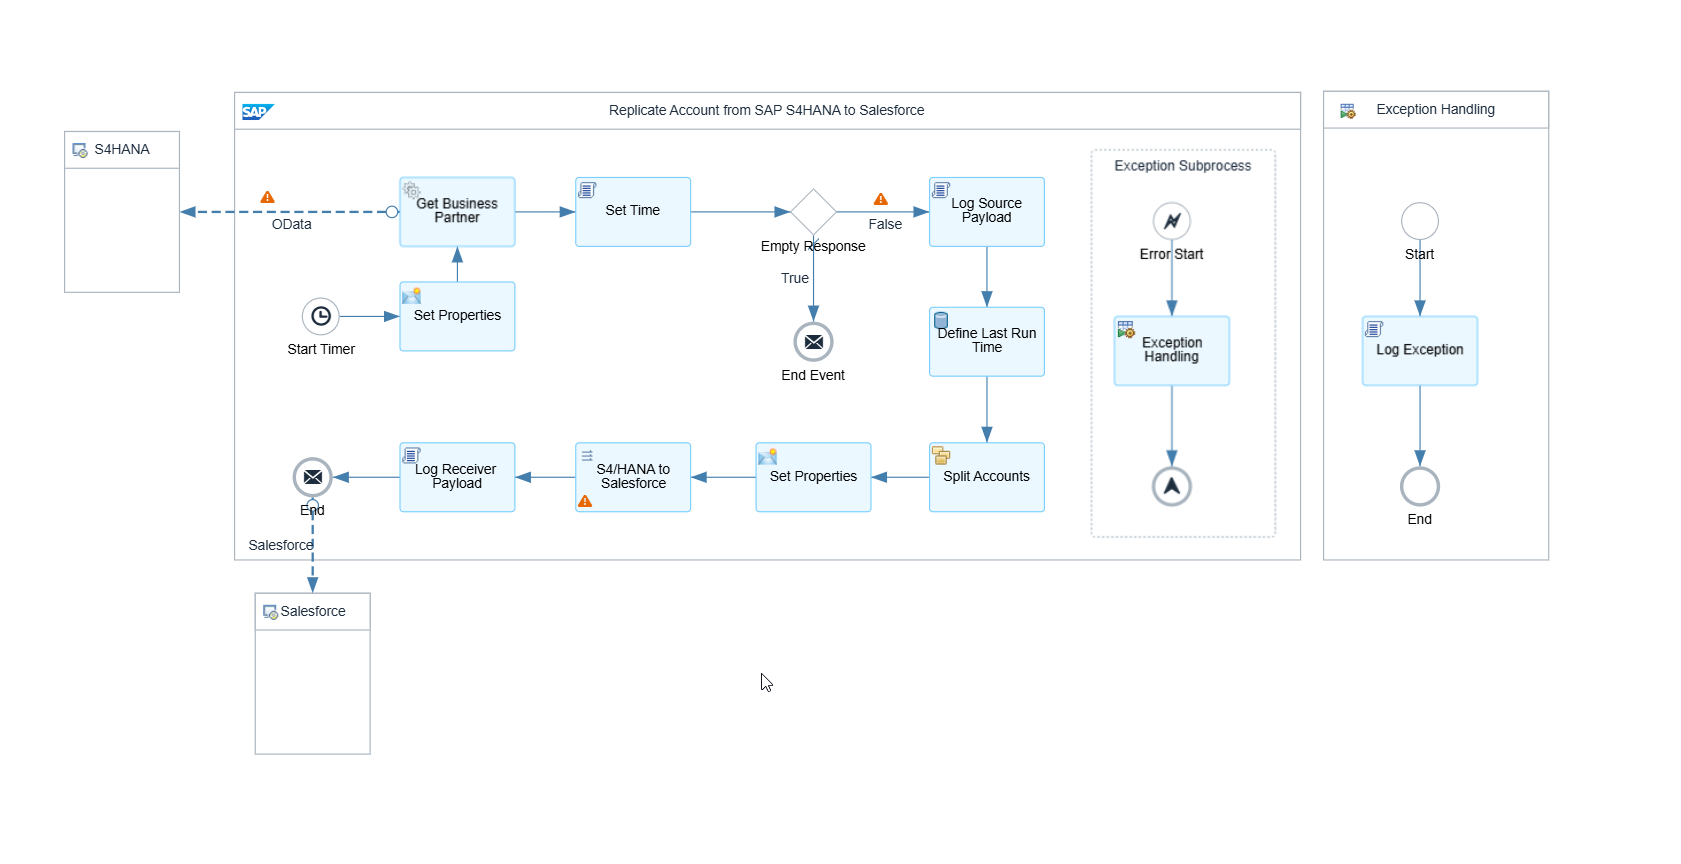
\includegraphics[width=0.8\textwidth]{Chapter4/Pictures/iflow.png}}
    \caption{Reference Field}
    
    \end{figure}


\paragraph{Prerequisites}
Before configuring the integration content, the following prerequisites must be addressed to ensure a smooth and successful implementation:

\begin{enumerate}
    \item \textbf{Deployment of Security Artifacts:}
    \begin{itemize}
        \item All necessary security artifacts, such as certificates, keys, and authentication tokens, must be deployed and configured. These artifacts are essential for establishing secure communication between SAP S/4HANA and Salesforce during the integration process.
    \end{itemize}

    
    \begin{figure}[H]
    \centering
    \fbox{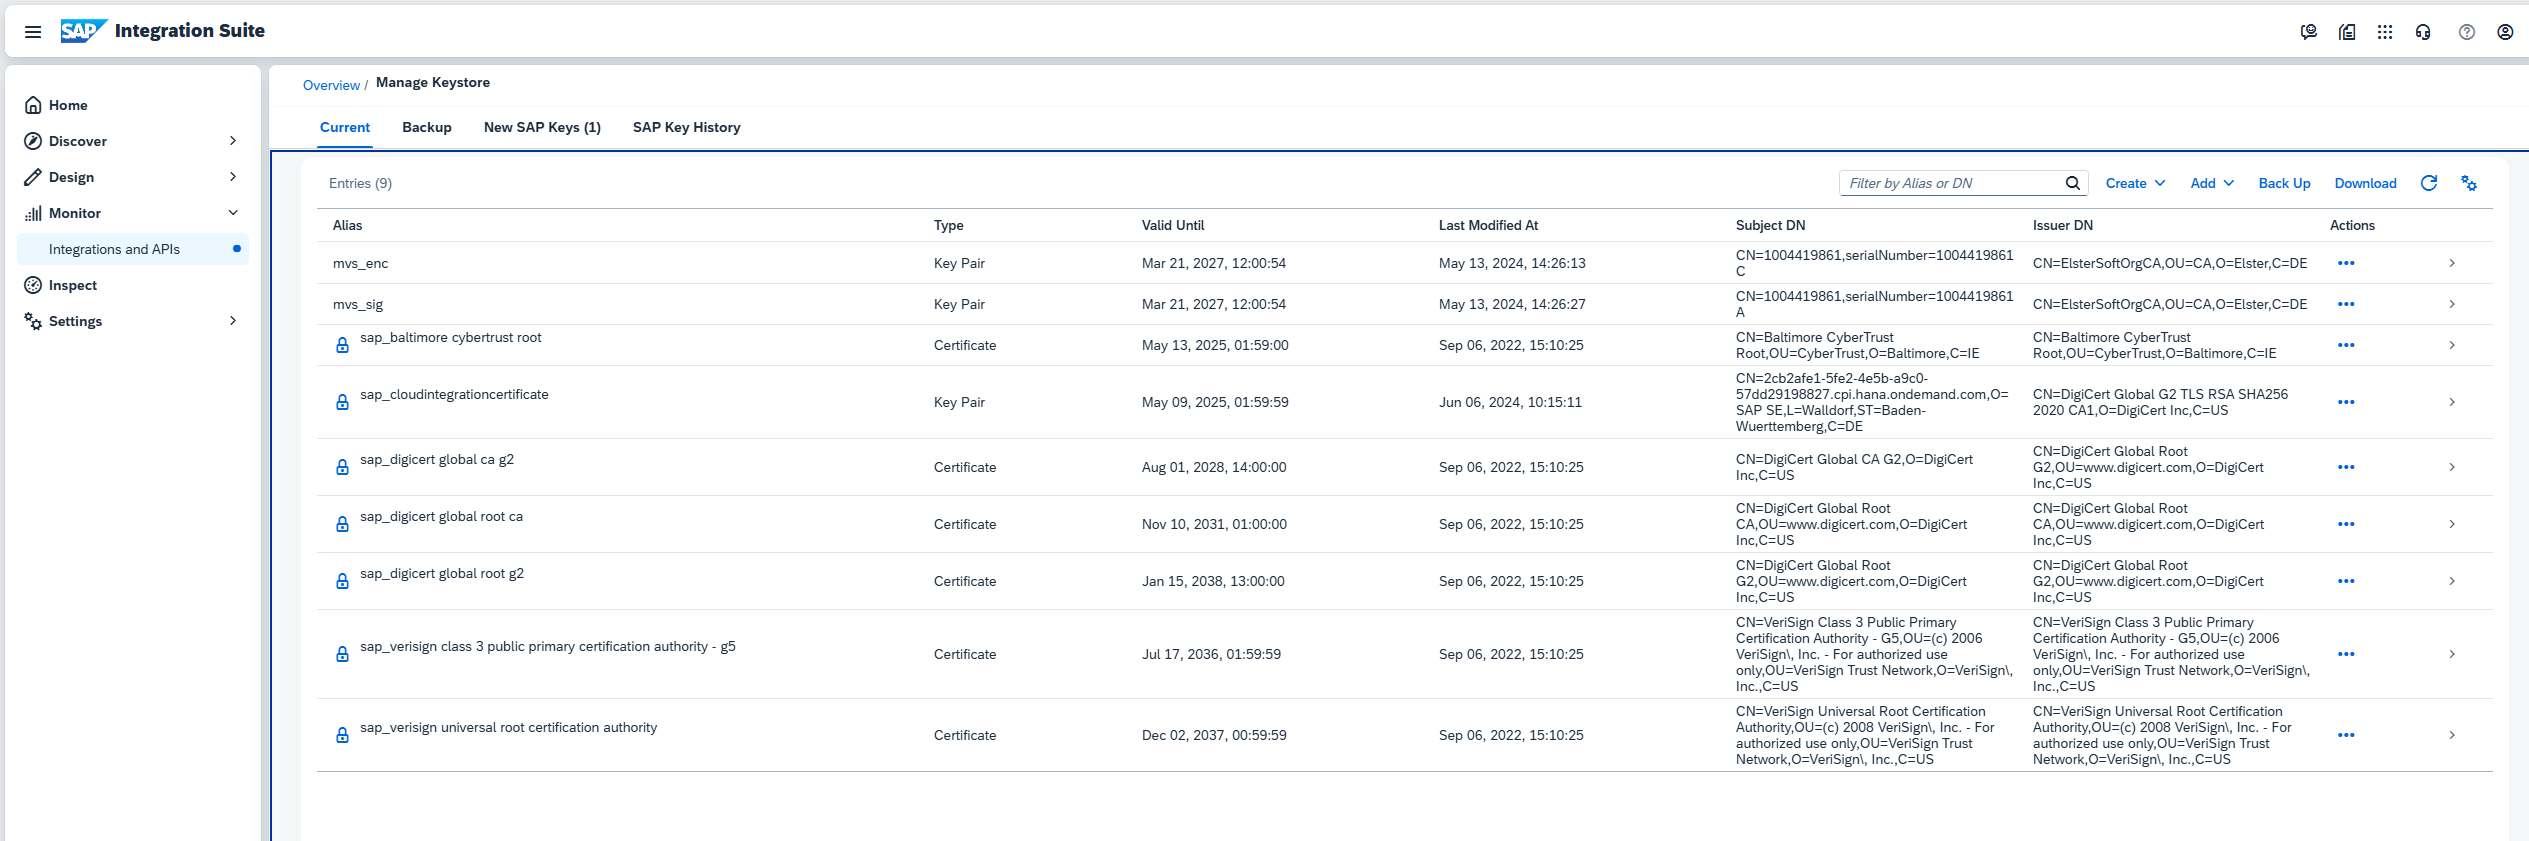
\includegraphics[width=0.8\textwidth]{Chapter4/Pictures/keys_certi.png}}
    \caption{Keys and Certificates in SAP Integration Suite}
    
    \end{figure}

    
    \begin{figure}[H]
    \centering
    \fbox{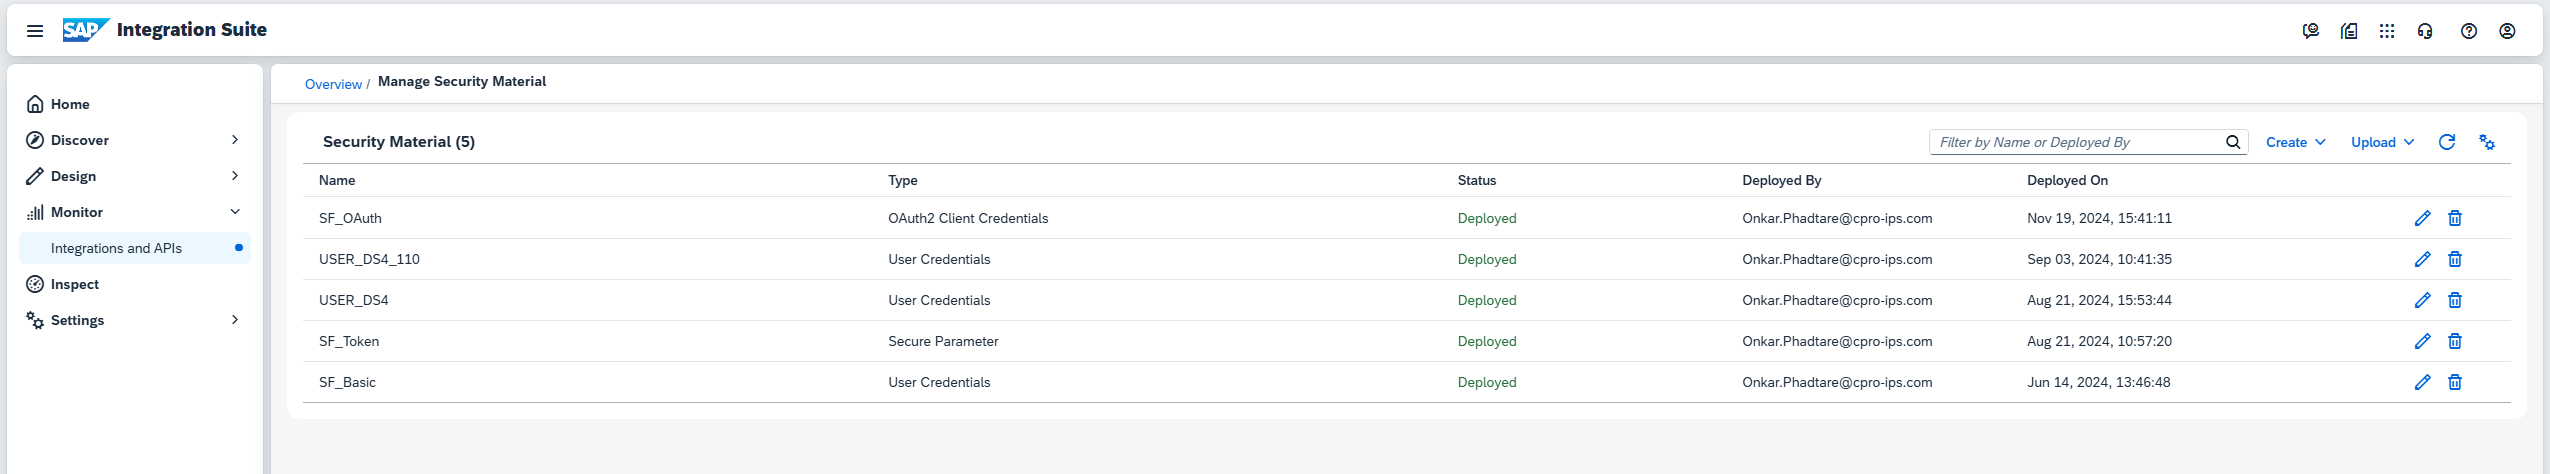
\includegraphics[width=0.8\textwidth]{Chapter4/Pictures/UserCred.png}}
    \caption{User Credentials in SAP Integration Suite}
    
    \end{figure}

    \item \textbf{Configuration of Time Zone and Initial Run Schedule:}
    \begin{itemize}
        \item Users must define the time zone in the configuration settings to ensure accurate scheduling and data replication. Additionally, the first run date and hour must be specified to determine when the integration flow should begin replicating data. This ensures that the replication process starts at the desired time and operates in the correct time context.
    \end{itemize}
\end{enumerate}

By fulfilling these prerequisites, the integration flow can be configured effectively, ensuring secure and timely replication of customer data from SAP S/4HANA to Salesforce.


\paragraph{Scope}
It is important to note that this integration flow is specifically designed to replicate Business Partners categorized as Customers from SAP S/4HANA to Salesforce. Business Partners belonging to other categories, such as vendors or suppliers, will not be included in the replication process. This ensures that only relevant customer data is synchronized between the two systems, maintaining data accuracy and alignment with the intended use case. The integration flow focuses exclusively on customer-related Business Partners, enabling efficient and targeted data replication for customer management in Salesforce.

\paragraph{Procedure } 

This section provides a step-by-step guide to configure the integration flow titled \textbf{"Replicate Account from SAP S/4HANA to Salesforce"}. The configuration process involves setting up the timer, configuring the receiver connectors for both SAP S/4HANA and Salesforce, and defining additional parameters under the "More" options. Below is a detailed explanation of each step:

\begin{enumerate}
    \item \textbf{Open the Integration Flow:}
    \begin{itemize}
        \item Begin by opening the integration flow \textbf{"Replicate Account from SAP S/4HANA to Salesforce"} in the SAP Cloud Platform Integration (CPI) interface. Click on the \textbf{Configure} button to proceed with the setup.
    \end{itemize}

    \begin{figure}[H]
    \centering
    \fbox{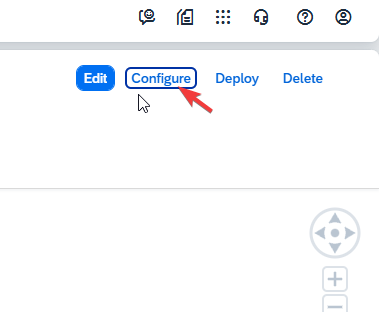
\includegraphics[width=0.8\textwidth]{Chapter4/Pictures/Configureiflow.png}}
    \caption{Configure the iFlow with Configure button}
    
    \end{figure}

    \item \textbf{Configure the Timer:}
    \begin{itemize}
        \item The timer determines the execution schedule of the integration flow. You can choose from the following options:
        \begin{itemize}
            \item \textbf{Run Once:} Executes the integration flow only once, typically used for initial data loads.
            \item \textbf{Schedule on Day:} Executes the integration flow on a specific date and time.
            \item \textbf{Schedule to Recur:} Executes the integration flow at regular intervals, ensuring continuous replication of changes from SAP S/4HANA to Salesforce. This is the recommended mode for ongoing synchronization.
        \end{itemize}
        \item Replace the default timer parameters with values appropriate for your specific scenario and system landscape.
    \end{itemize}

    \begin{figure}[H]
    \centering
    \fbox{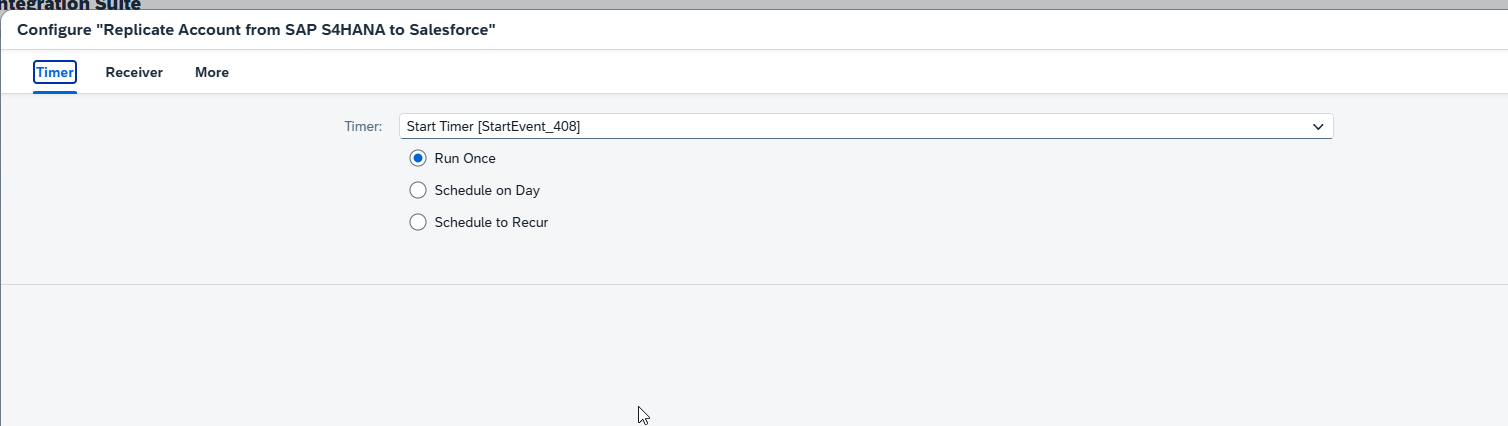
\includegraphics[width=0.8\textwidth]{Chapter4/Pictures/Schedule.png}}
    \caption{Timer Configuration in SAP Integration Suite}
    
    \end{figure}

    \item \textbf{Configure the SAP S/4HANA Receiver Connector:}
    \begin{itemize}
        \item Navigate to the \textbf{Receiver} section and configure the connector named \textbf{"S4HANA"}. The following parameters must be defined:
        \begin{itemize}
            \item \textbf{Hostname:} Enter the API hostname of your SAP S/4HANA system (e.g., \texttt{https://hostname:port/sap/opu/odata/sap/API\_BUSINESS\_PARTNER}).
            \item \textbf{Port:} Specify the API port of your SAP S/4HANA system.
            \item \textbf{Location ID:} Provide the location identifier for your SAP S/4HANA tenant.
            \item \textbf{Credential Name:} Enter the name of the credential artifact deployed for SAP S/4HANA authentication.
        \end{itemize}
    \end{itemize}


    \begin{figure}[H]
    \centering
    \fbox{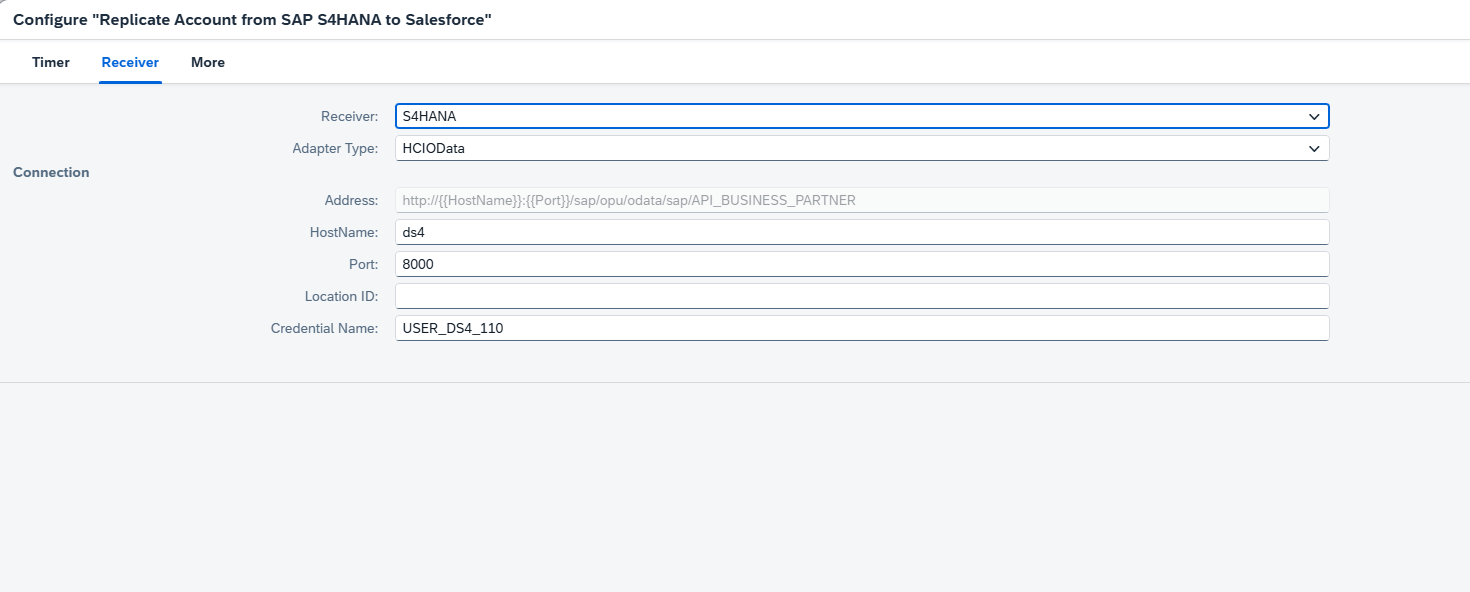
\includegraphics[width=0.8\textwidth]{Chapter4/Pictures/RecieverS4.png}}
    \caption{Receiver Configuration for SAP S/4HANA in SAP Integration Suite:}
    
    \end{figure}

    \item \textbf{Configure the Salesforce Receiver Connector:}
    \begin{itemize}
        \item Configure the connector named \textbf{"Salesforce"} with the following parameters:
        \begin{itemize}
            \item \textbf{Address:} Enter the data store URL for Salesforce (e.g., \texttt{https://login.salesforce.com}).
            \item \textbf{Basic Credential Name:} Specify the name of the deployed user credentials artifact containing the username and password for Salesforce authentication.
            \item \textbf{Security Token Alias:} Provide the name of the deployed secure parameter artifact holding the Salesforce security token, required for untrusted network access.
            \item \textbf{OAuth Credential Name:} Enter the name of the deployed OAuth credential artifact, if applicable.
        \end{itemize}
    \end{itemize}

    \begin{figure}[H]
    \centering
    \fbox{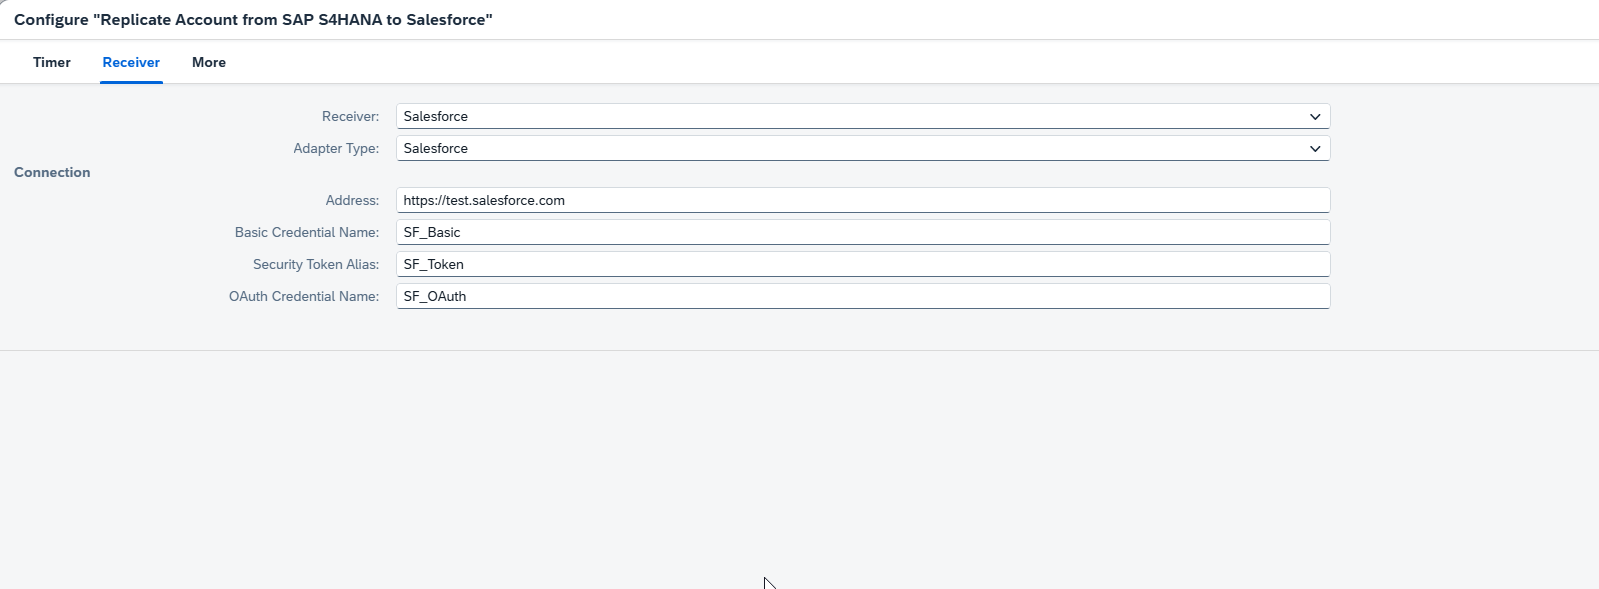
\includegraphics[width=0.8\textwidth]{Chapter4/Pictures/RecieverSF.png}}
    \caption{Receiver Configuration for Salesforce in SAP Integration Suite}
    
    \end{figure}

    \item \textbf{Configure Additional Options Under "More":}
    \begin{itemize}
        \item Under the \textbf{"More"} section, configure the following parameters:
        \begin{itemize}
            \item \textbf{ExceptionLogging:} Set to \textbf{"YES"} to log exceptions or \textbf{"NO"} to disable logging.
            \item \textbf{InitialDate:} Specify the start date for replication in the format \texttt{YYYY-MM-DD’T’hh:mm:ss.sss’Z’} (e.g., \texttt{1970-01-01T00:00:00.000Z}).
            \item \textbf{InitialHour:} Define the start time for replication in the format \texttt{‘PT’hh’H’mm’M’ss’S’} (e.g., \texttt{PT00H00M00S}).
            \item \textbf{LogMessageBody:} Set to \textbf{"YES"} to log the message body (not recommended for live environments) or \textbf{"NO"} to disable.
            \item \textbf{LogMessageHeader:} Set to \textbf{"YES"} to log the message header or \textbf{"NO"} to disable.
            \item \textbf{LogMessageProperty:} Set to \textbf{"YES"} to log message properties or \textbf{"NO"} to disable.
        \end{itemize}
    \end{itemize}

    \begin{figure}[H]
    \centering
    \fbox{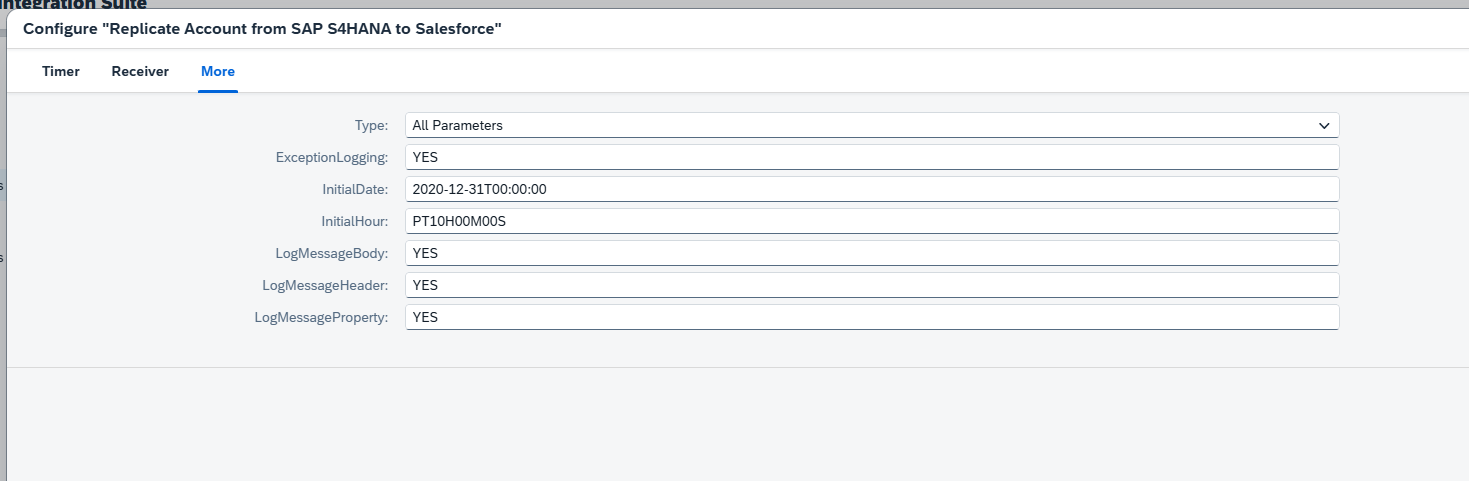
\includegraphics[width=0.8\textwidth]{Chapter4/Pictures/More.png}}
    \caption{Additional Configuration Settings in SAP Integration Suite}
    
    \end{figure}

    \item \textbf{Save and Deploy:}
    \begin{itemize}
        \item After completing the configuration, save the settings and deploy the integration flow. This activates the flow, enabling it to replicate customer data from SAP S/4HANA to Salesforce based on the defined schedule and parameters.
    \end{itemize}
\end{enumerate}


    \begin{figure}[H]
    \centering
    \fbox{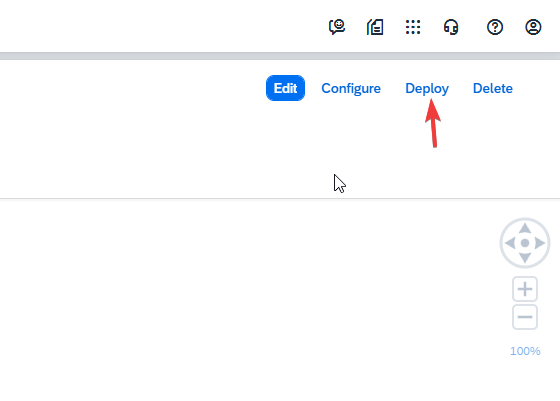
\includegraphics[width=0.8\textwidth]{Chapter4/Pictures/savedeploy.png}}
    \caption{Deploying the Integration Artifact in SAP Integration Suite}
    
    \end{figure}


This configuration process ensures that the integration flow operates efficiently, maintaining data consistency and alignment between SAP S/4HANA and Salesforce.




%=== END OF CHAPTER FOUR ===
\newpage